\documentclass[11pt]{article}

\usepackage[margin=1in]{geometry}
\usepackage{setspace}
\onehalfspacing
\usepackage{graphicx}
\graphicspath{report_images/}
\usepackage{appendix}
\usepackage{listings}
\usepackage{float}
\usepackage{multirow}
\usepackage{amsthm}
% The next three lines make the table and figure numbers also include section number
\usepackage{chngcntr}
\counterwithin{table}{section}
\counterwithin{figure}{section}
% Needed to make titling page without a page number
\usepackage{titling}

% DOCUMENT INFORMATION =================================================
\font\titleFont=cmr12 at 11pt
\title {{\titleFont ECEN 429: Introduction to Digital Systems Design Laboratory \\ North Carolina Agricultural and Technical State University \\ Department of Electrical and Computer Engineering}} % Declare Title
\author{\titleFont Reporter: Nikiyah Beulah\\ \titleFont Partner: Chris Cannon} % Declare authors
\date{\titleFont March 1, 2018}
% ======================================================================

\begin{document}

\begin{titlingpage}
\maketitle
\begin{center}
	Lab 6
\end{center}
\end{titlingpage}

\section{Introduction}
The object of this lab is to implement two different types of state machines, Mealy and Moore. State machines are defined in Definition ~\ref{def:state_machine}. State machines are useful for a wide range of applications, most basically as a sequence detector. Sequence detectors are state machines that will output '1' or HIGH when a set sequence of inputs is detected.

\theoremstyle{definition}
\newtheorem{definition}{Definition}
\begin{definition}
State Machine: A device that can be in one of a set number of stable conditions depending on its previous condition and on the present values of its inputs.
\label{def:state_machine}
\end{definition}

\section{Background, Design Solution, and Results}

\subsection{Problem 1 }

\subsubsection{Background}
Our first task in the lab was not to implement a state machine directly. Rather, the first task was to implement a clock divider that will slow down the frequency of the clock to a speed that a human can work with. In order to implement and test our sequence detectors, we will need time to provide the inputs between each clock cycle. The Basys3 board has a 100 MHz clock, and our task for this lab was to slow it down as low as 1 Hz.

\subsubsection{Design Solution}
In order to reduce the clock speed from 100 MHz, or 100,000,000 Hz, to approximately 1 Hz, we had to derive the approximate number of clock cycles it will take, and identify the number of bits used to represent that value. Equation ~\ref{eqn:decimal_to_binary} shows the conversion to a 27 bit binary number. Once we knew that the number was 27 bits, we plugged 27 into the provided code. The port assignments used for the clock divider are summarized in Table ~\ref{tab:clockDivider_input_Ports}.

\begin{equation}
100 000 000d = 101111101011110000100000000b
\label{eqn:decimal_to_binary}
\end{equation}

\begin{table}[H]
\begin{center}
\begin{tabular}{| l | l | l |}
	\hline
	Bit & Label & Port \\ \hline
	FastClock & LED 0 & U16 \\ \hline
	MediumClock & LED 1 & E19 \\ \hline
	SlowClock & LED 2 & U19 \\ \hline
	led0 & LED 15 & L1 \\ \hline
\end{tabular}
\caption{\label{tab:clockDivider_input_Ports}Input port assignments for Clock Divider.}
\end{center}
\end{table}

\begin{table}[H]
\begin{center}
\begin{tabular}{| l | l | l |}
	\hline
	Bit & Label & Port \\ \hline
	clk & Clock & W5 \\ \hline
	starttimer & Switch 0 & V17 \\ \hline
\end{tabular}
\caption{\label{tab:clockDivider_output_Ports}Output port assignments for Clock Divider.}
\end{center}
\end{table}

\subsubsection{Results}
The clock divider successfully slowed the clock signal from 100 MHz to 1 Hz, or 1 iteration per second. The functioning clock is shown in Figures ~\ref{fig:part1img1} through ~\ref{fig:part1img3}.

\begin{center}
\begin{figure}[H]
	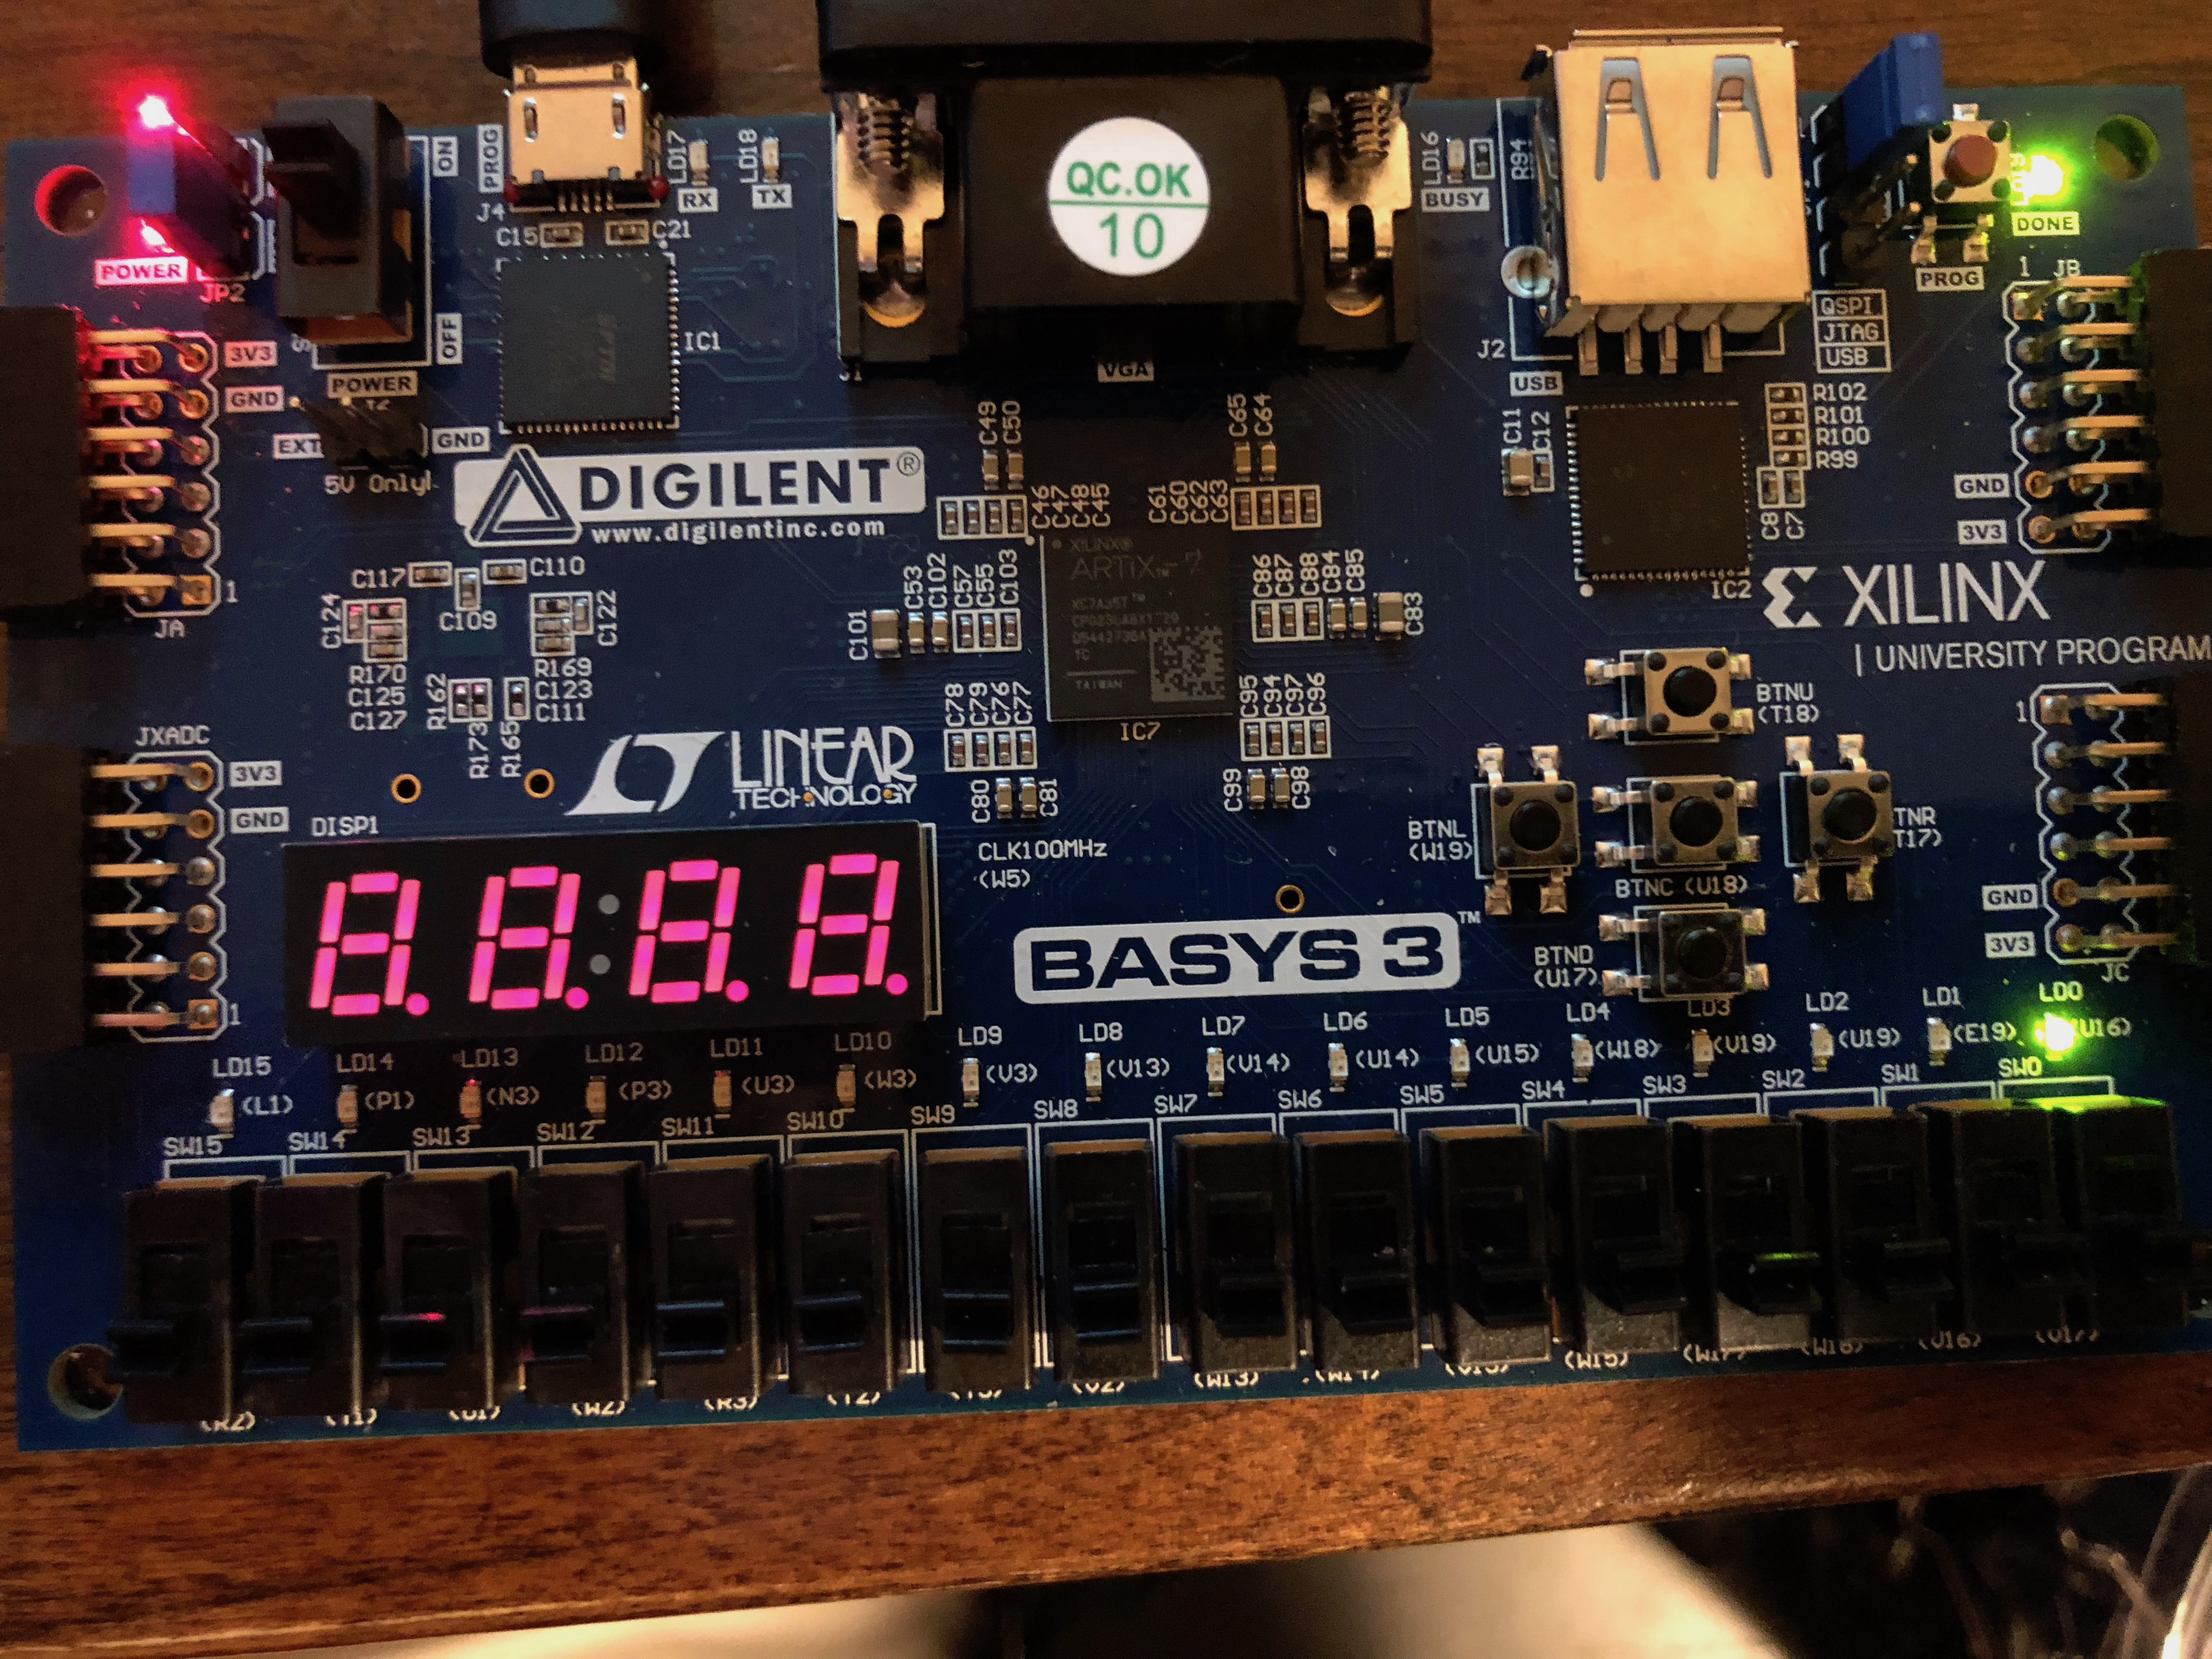
\includegraphics[width=0.5\textwidth]{./images/Part1/IMG_0574.jpg}
	\caption{\label{fig:part1img1}This image shows the clock that is currently not started. Switch 0 is off and therefore the lights are not flashing.}
\end{figure}
\end{center}

\begin{center}
\begin{figure}[H]
	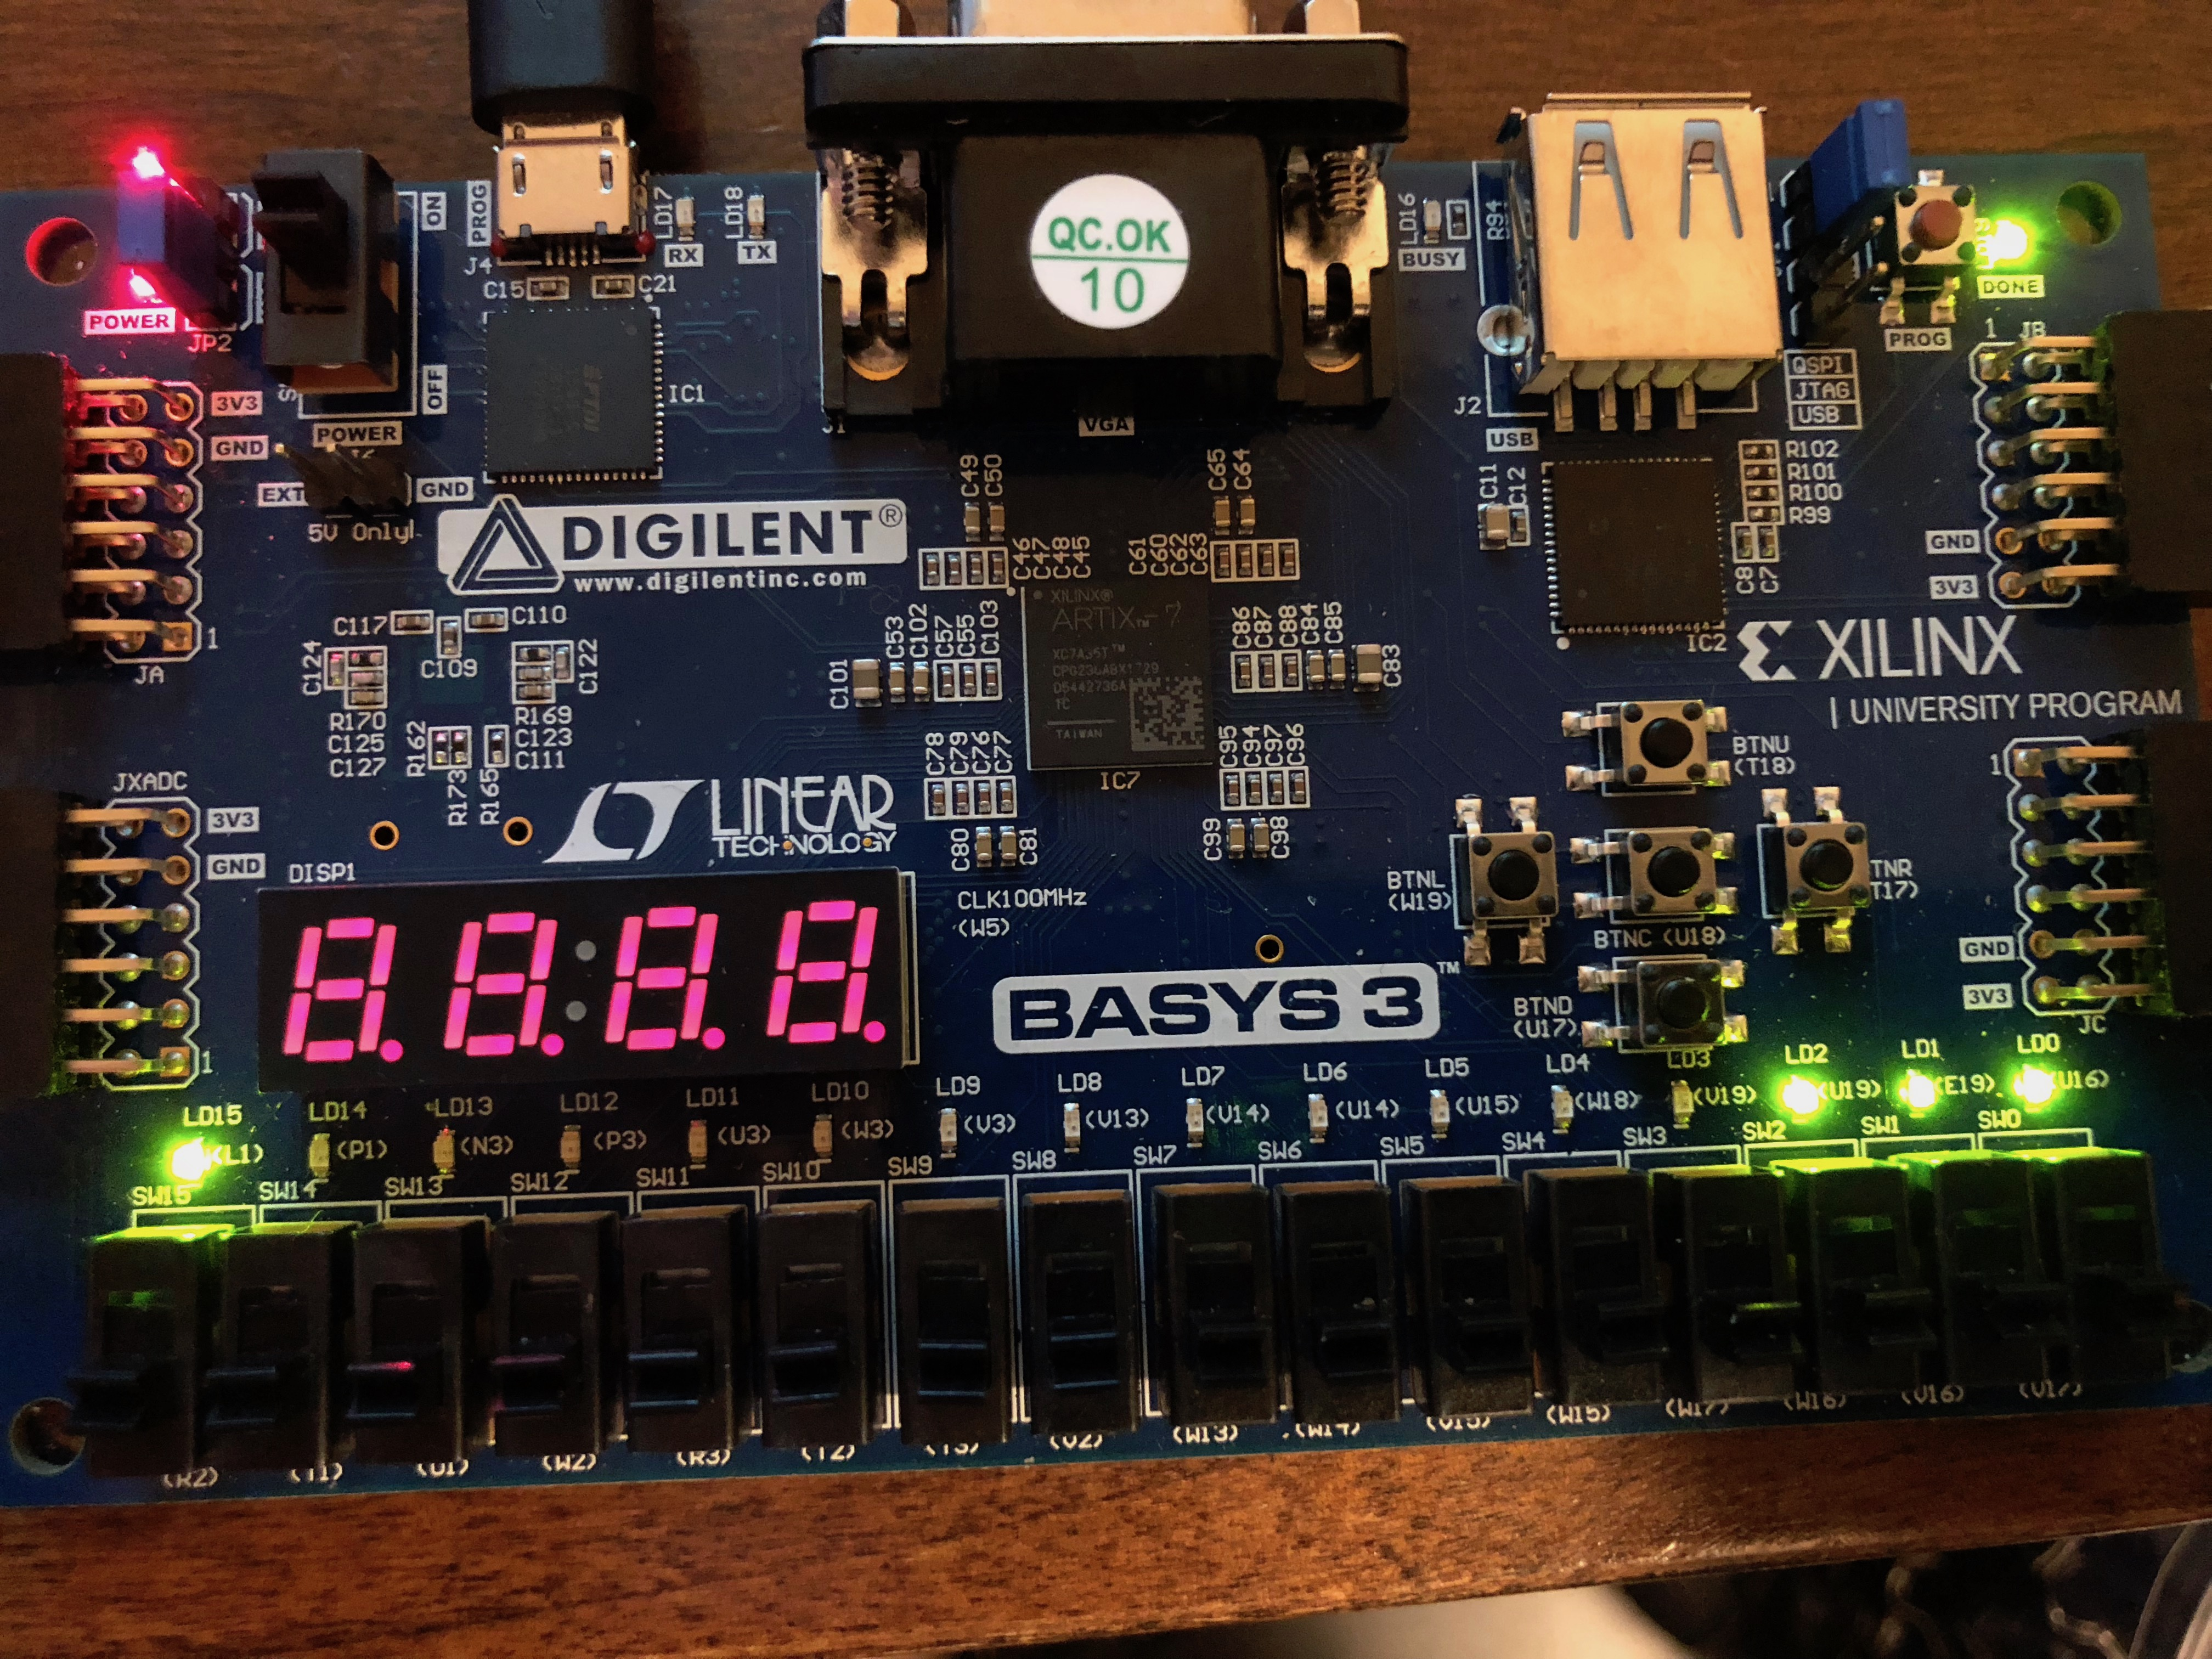
\includegraphics[width=0.5\textwidth]{./images/Part1/IMG_0575.jpg}
	\caption{\label{fig:part1img2}In this figure all three clock speeds are on. The LED on the left is an LED that coordinates with the SlowClock signal, and will be used in the state machines to help the user visualize the clock. }
\end{figure}
\end{center}

\begin{center}
\begin{figure}[H]
	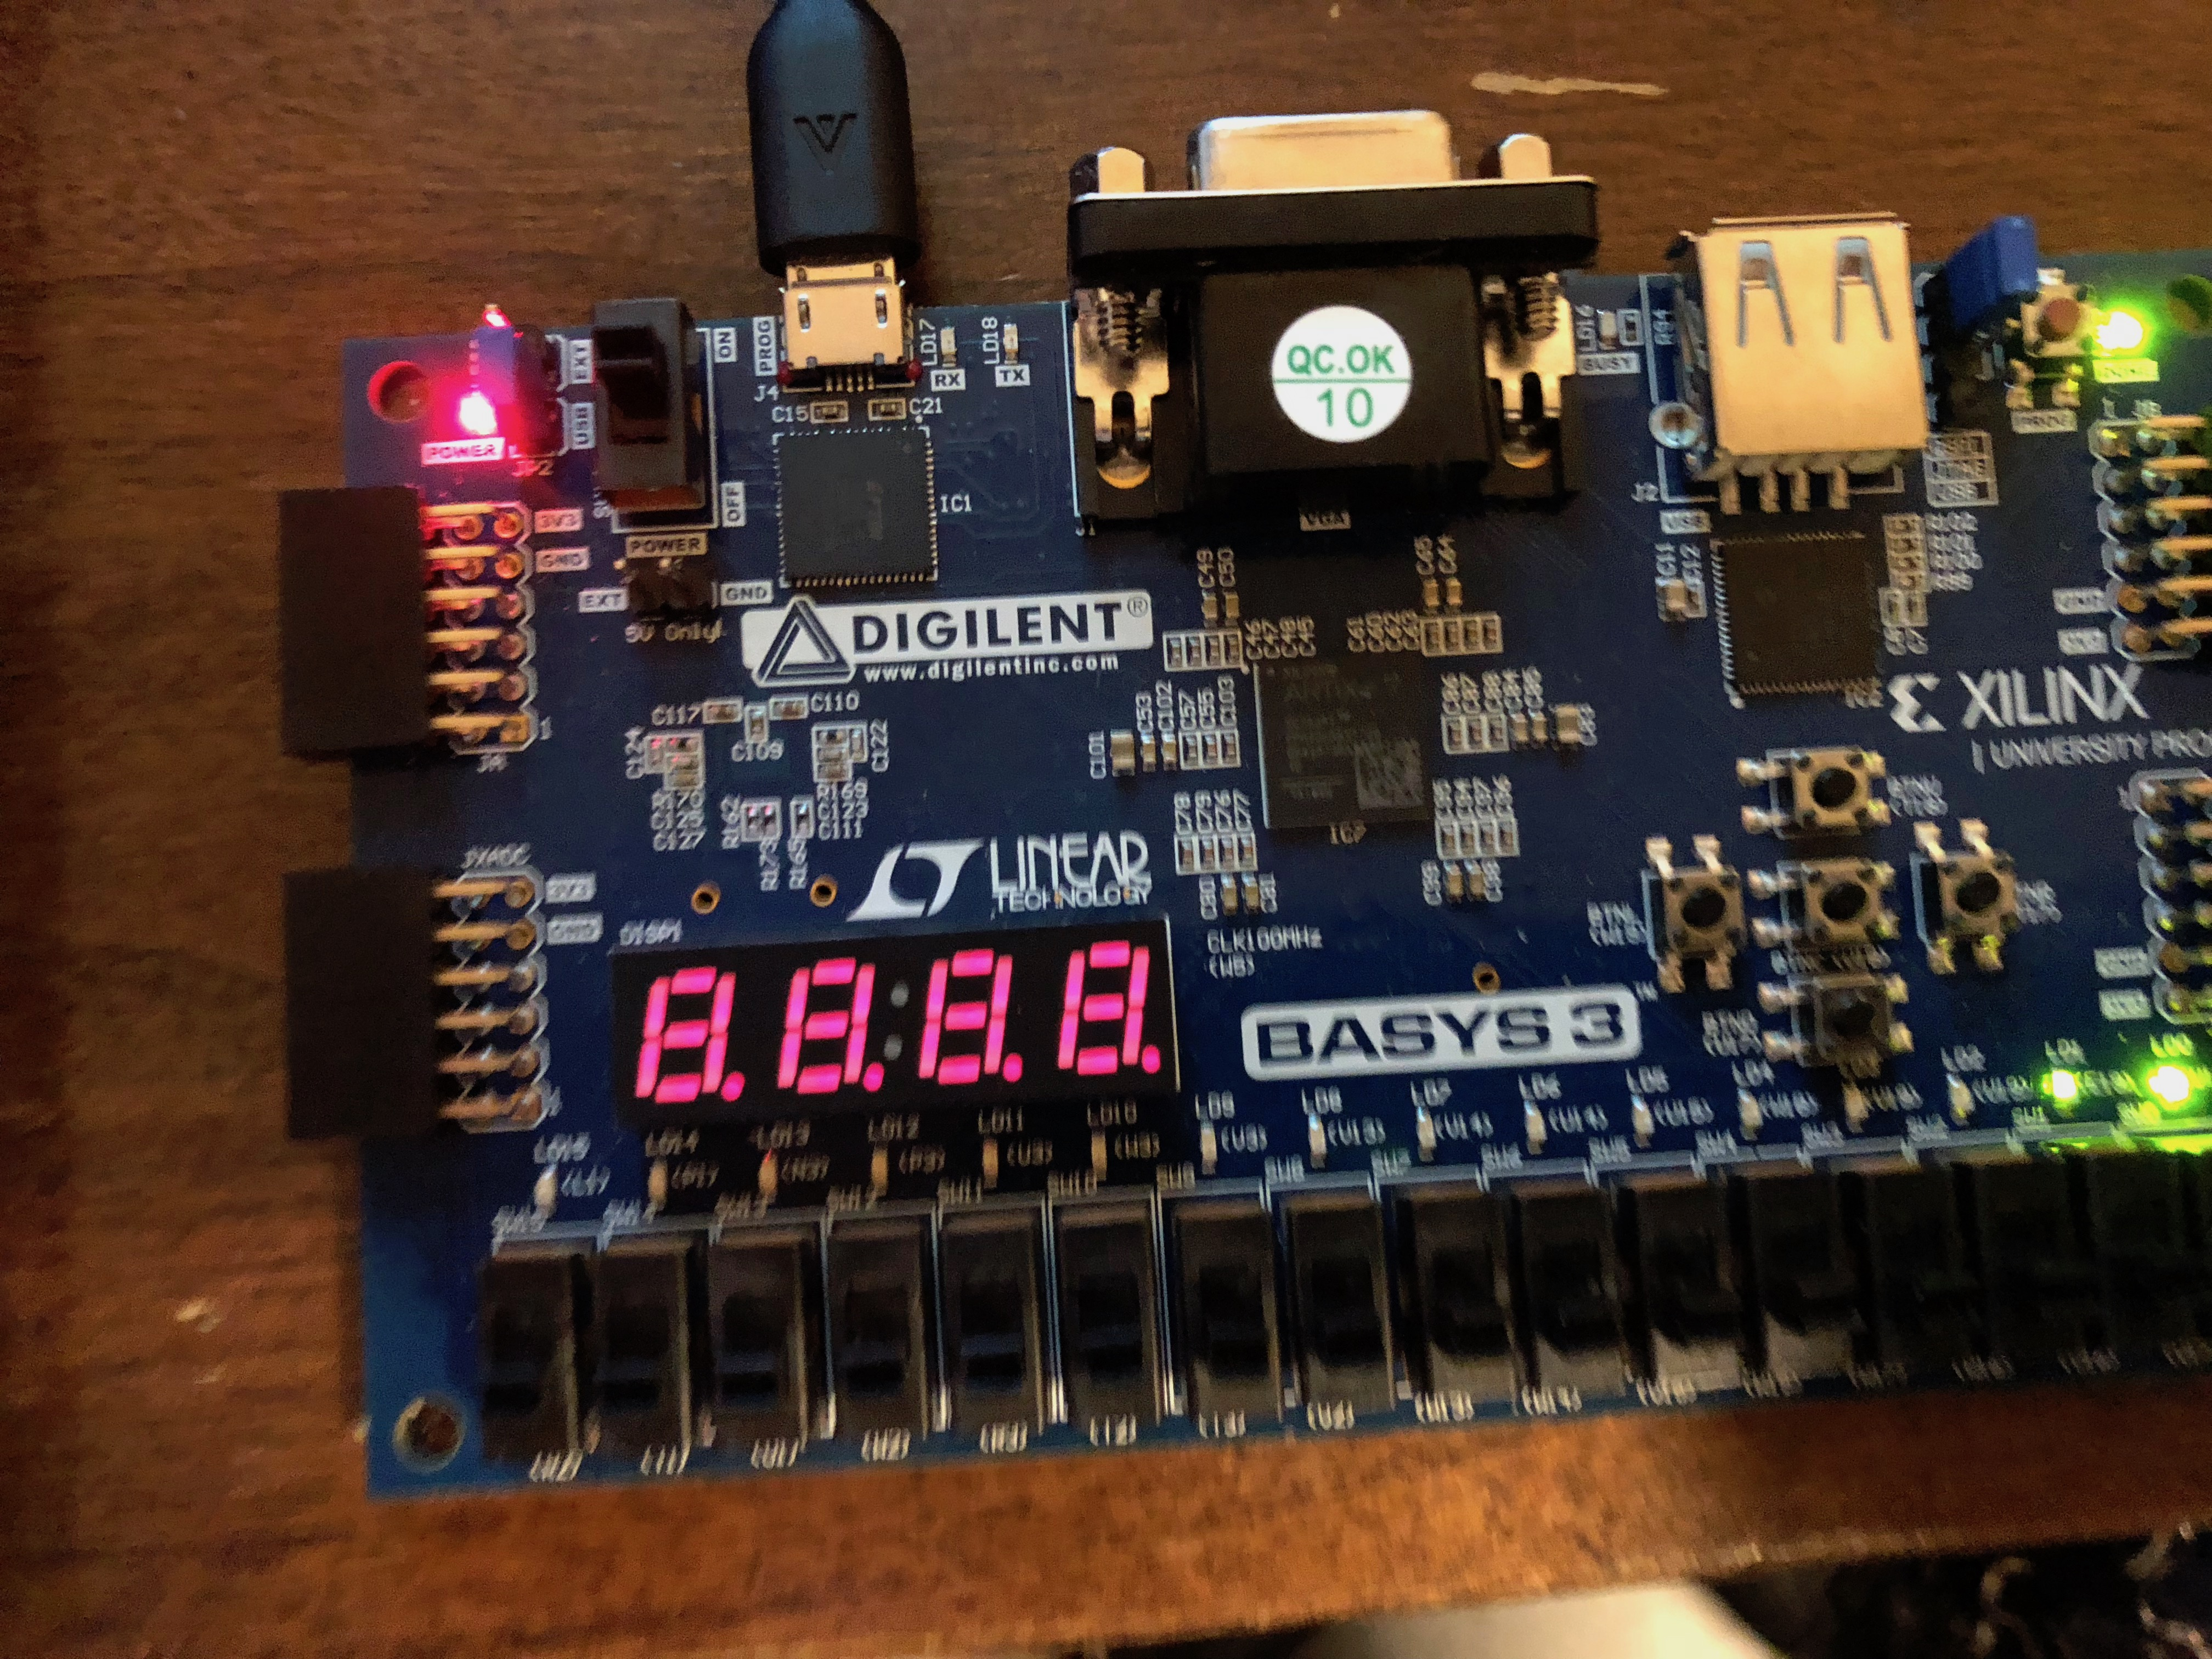
\includegraphics[width=0.5\textwidth]{./images/Part1/IMG_0577.jpg}
	\caption{\label{fig:part1img3}This image shows the differences between the 3 signals. Fast clock is LED 0 on the far right, it is fully on. MediumClock is LED 1 which is rising, and appears half-bright. SlowClock is represented by LED 2 and is off.}
\end{figure}
\end{center}

\subsection{Problem 2 }

\subsubsection{Background}
For Problem 2, we had to utilize our clock divider implemented in Problem 1 as we design and test a Moore State Machine. A Moore State Machine is one who's output depends only on the current state, not on the input. The inputs can be used to progress a Moore State Machine through its given states, but its output does not care what the input is. 

\subsubsection{Design Solution}
For our design, we had to implement a 10-state Moore Machine that would output '1' or HIGH at 2 states of our choice. For the purposed of this experiment, we selected state 4 and state 8. The state diagram is shown in Figure ~\ref{fig:moore_state_diagram}. Basically, this machine should progress through the states every clock cycle as long as the enable bit is '1' or HIGH. When it reaches state 9, it should return to state 0. The ports for this design are summarized in Tables ~\ref{tab:moore_input_ports} and ~\ref{tab:moore_output_ports}.

\begin{center}
\begin{figure}[H]
	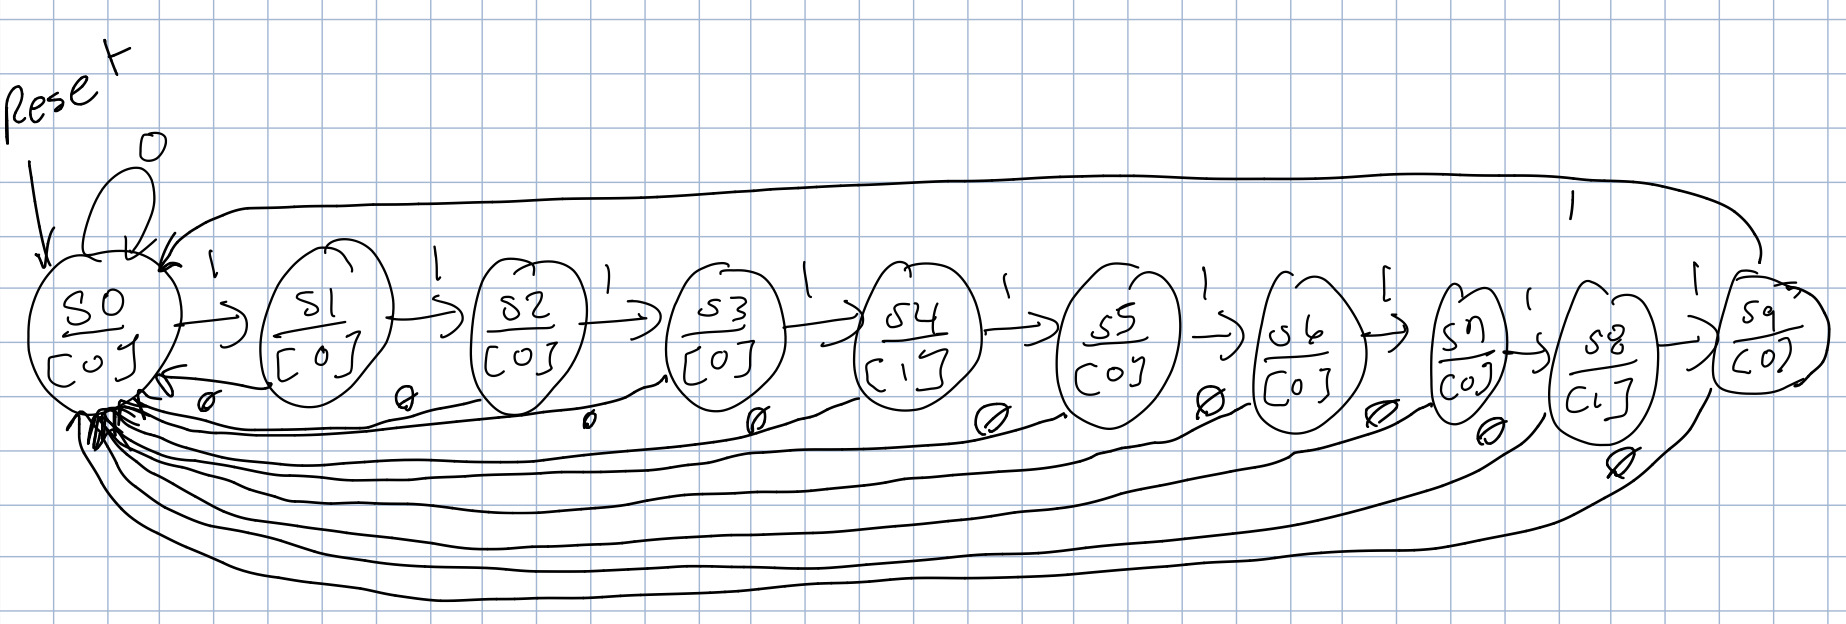
\includegraphics[width=\textwidth]{images/img1.jpg}
	\caption{\label{fig:moore_state_diagram}Moore State Diagram showing output at states 4 and 8.}
\end{figure}
\end{center}

\begin{table}[H]
\begin{center}
\begin{tabular}{| l | l | l |}
	\hline
	Bit & Label & Port \\ \hline
	clk & Clock & W5 \\ \hline
	enable & Switch 0 & V17 \\ \hline
	input & Switch 1 & U18 \\ \hline
\end{tabular}
\caption{\label{tab:moore_input_ports}Input port assignments for the Moore State Machine.}
\end{center}
\end{table}

\begin{table}[H]
\begin{center}
\begin{tabular}{| l | l | l |}
	\hline
	led0 & LED 15 & L1 \\ \hline
	state0 & LED 0 & U16 \\ \hline
	state1 & LED 1 & E19 \\ \hline
	state2 & LED 2 & U19 \\ \hline
	state3 & LED 3 & V19 \\ \hline
	state4 & LED 4 & W18 \\ \hline
	state5 & LED 5 & U15 \\ \hline
	state6 & LED 6 & U14 \\ \hline
	state7 & LED 7 & V14 \\ \hline
	state8 & LED 8 & V13 \\ \hline
	state9 & LED 9 & V3 \\ \hline
	output0 & Segment A & W7 \\ \hline
	output1 & Segment B & W6 \\ \hline
	output2 & Segment C & U8 \\ \hline
	output3 & Segment D & V8 \\ \hline
	output4 & Segment E & U5 \\ \hline
	output5 & Segment F & V5 \\ \hline
	output6 & Segment G & U7 \\ \hline
\end{tabular}
\caption{\label{tab:moore_output_ports}Output port assignments for the Moore State Machine.}
\end{center}
\end{table}

\subsubsection{Results}
The state machine successfully progressed through the states and output '1' in states 4 and 8. Some example outputs of the Moore State Machine are shown in Figures ~\ref{fig:part2img1} through ~\ref{fig:part2img5}.

\begin{center}
\begin{figure}[H]
	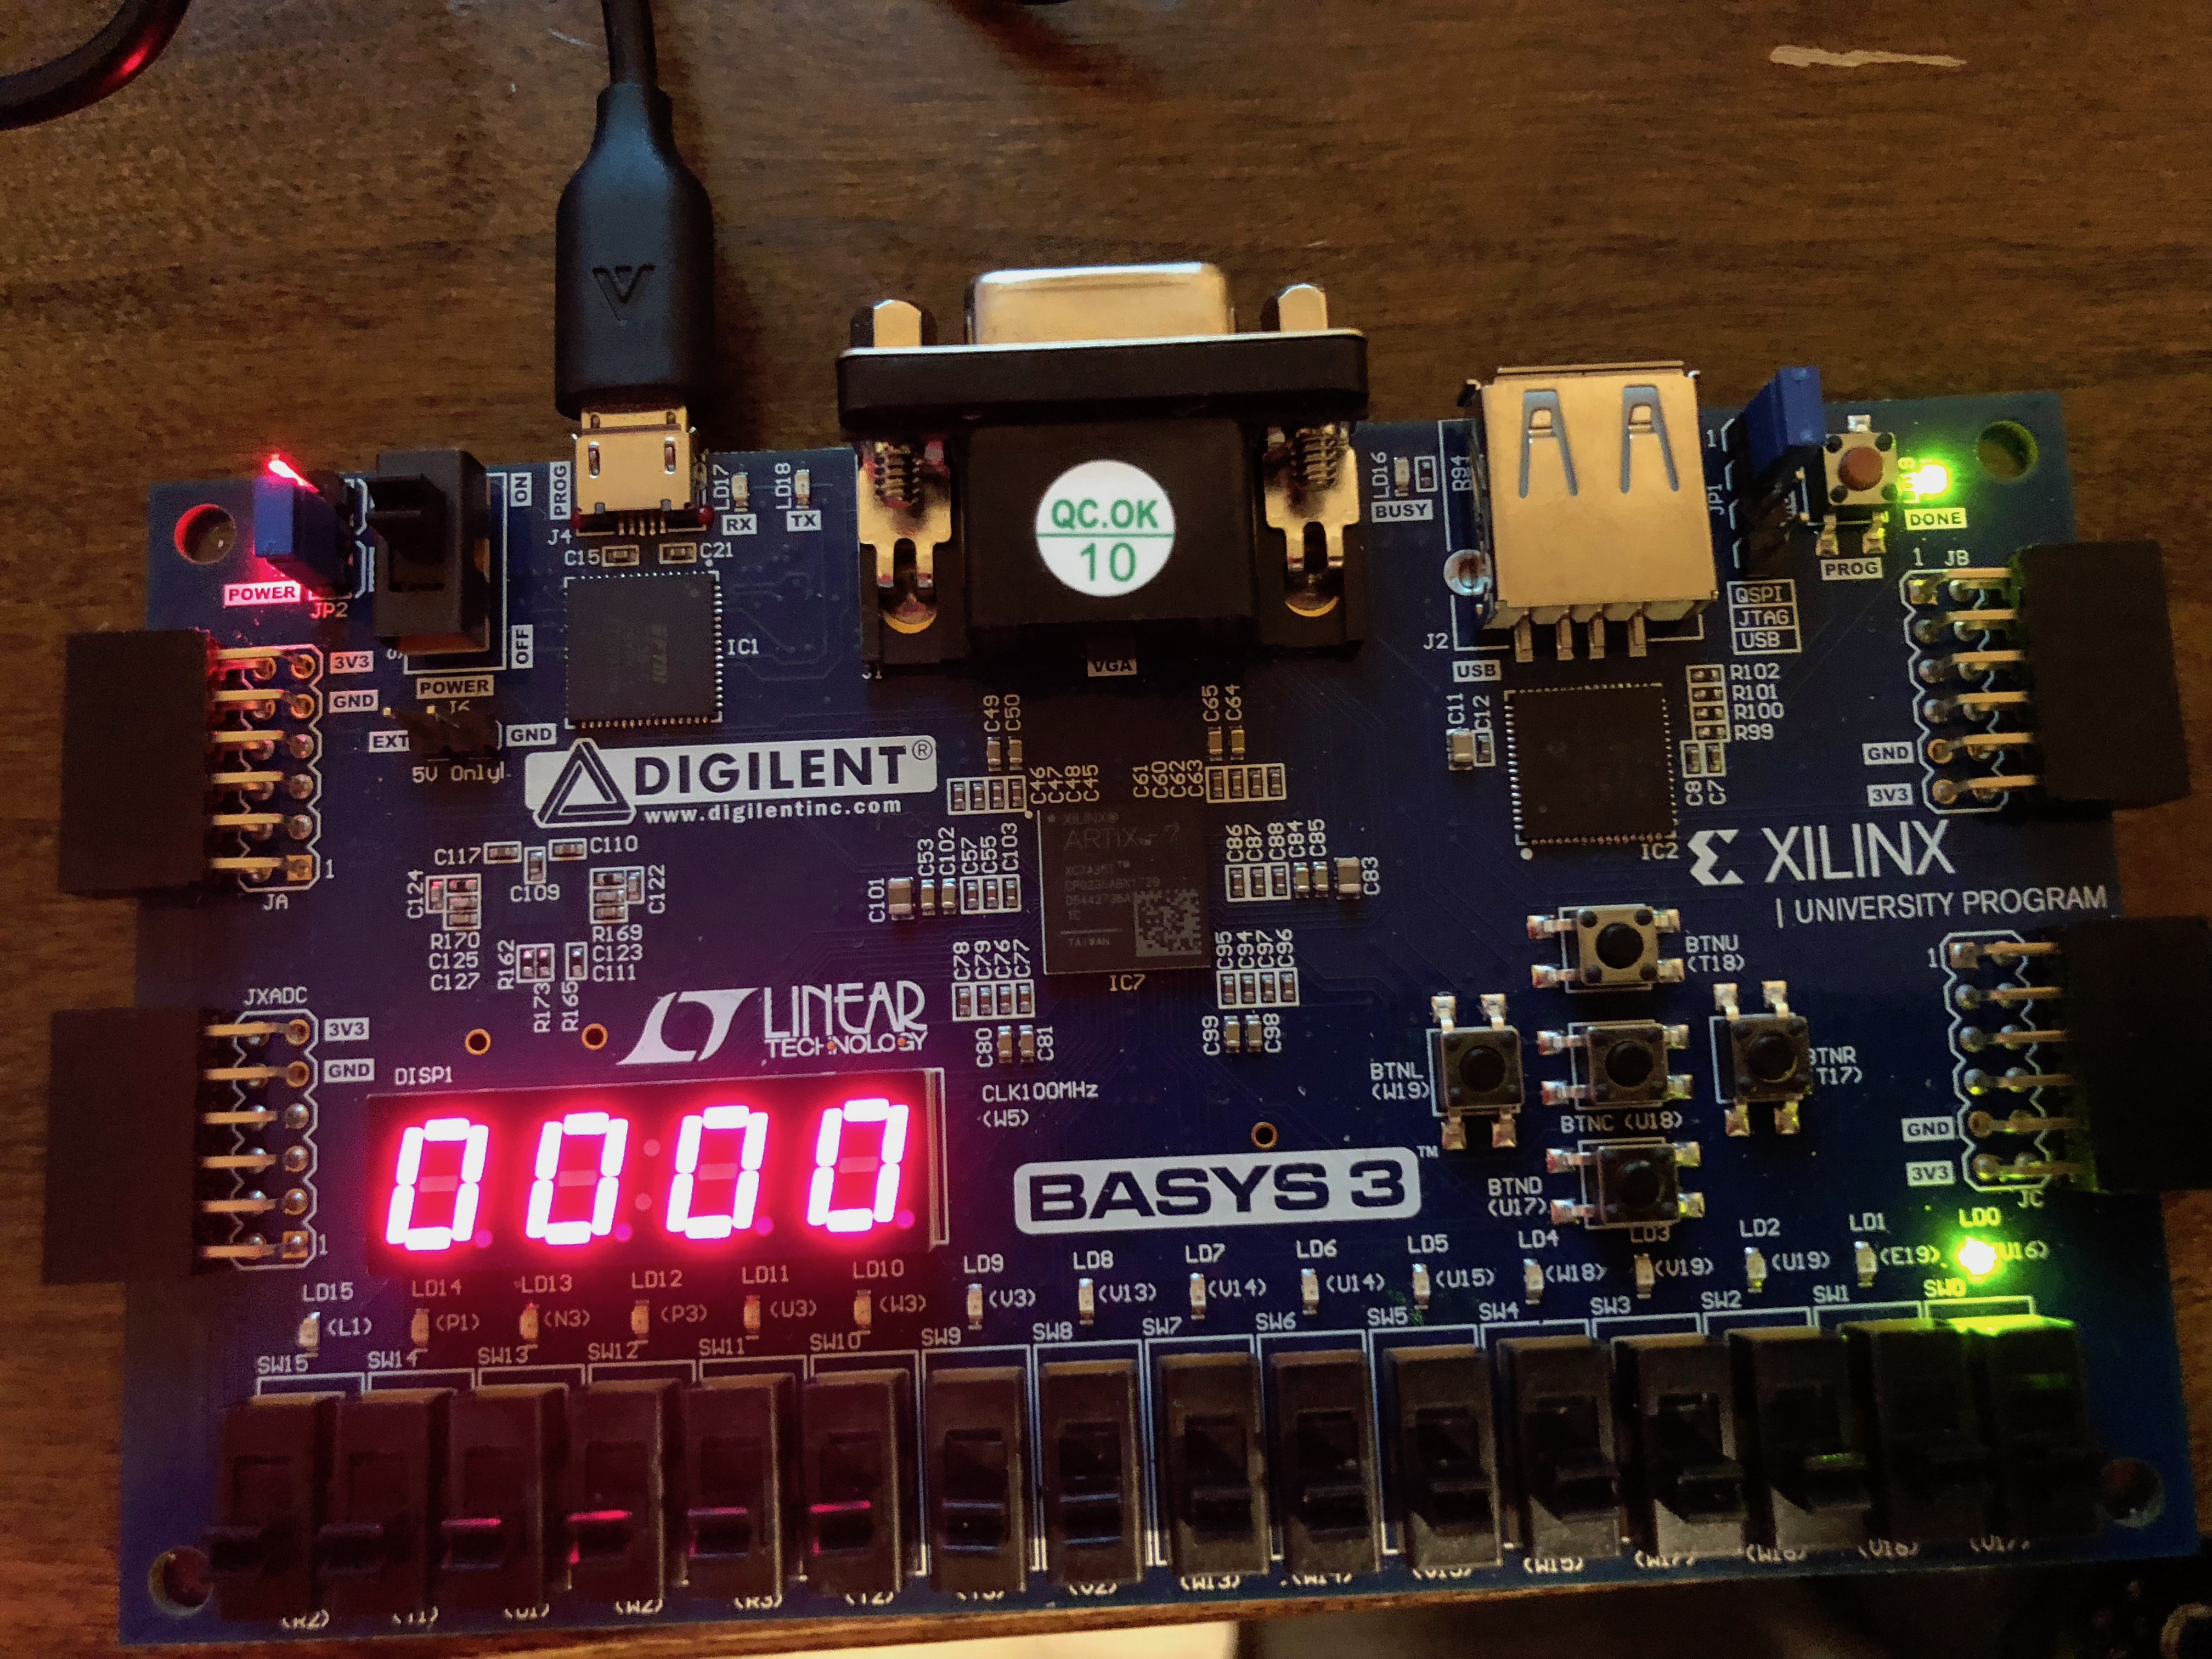
\includegraphics[width=0.5\textwidth]{./images/Part2/IMG_0578.jpg}
	\caption{\label{fig:part2img1}This image shows the state machine with a '0' input. Therefor, it will remain in State 0 with an output of 0 because Switch 0 is off.}
\end{figure}
\end{center}

\begin{center}
\begin{figure}[H]
	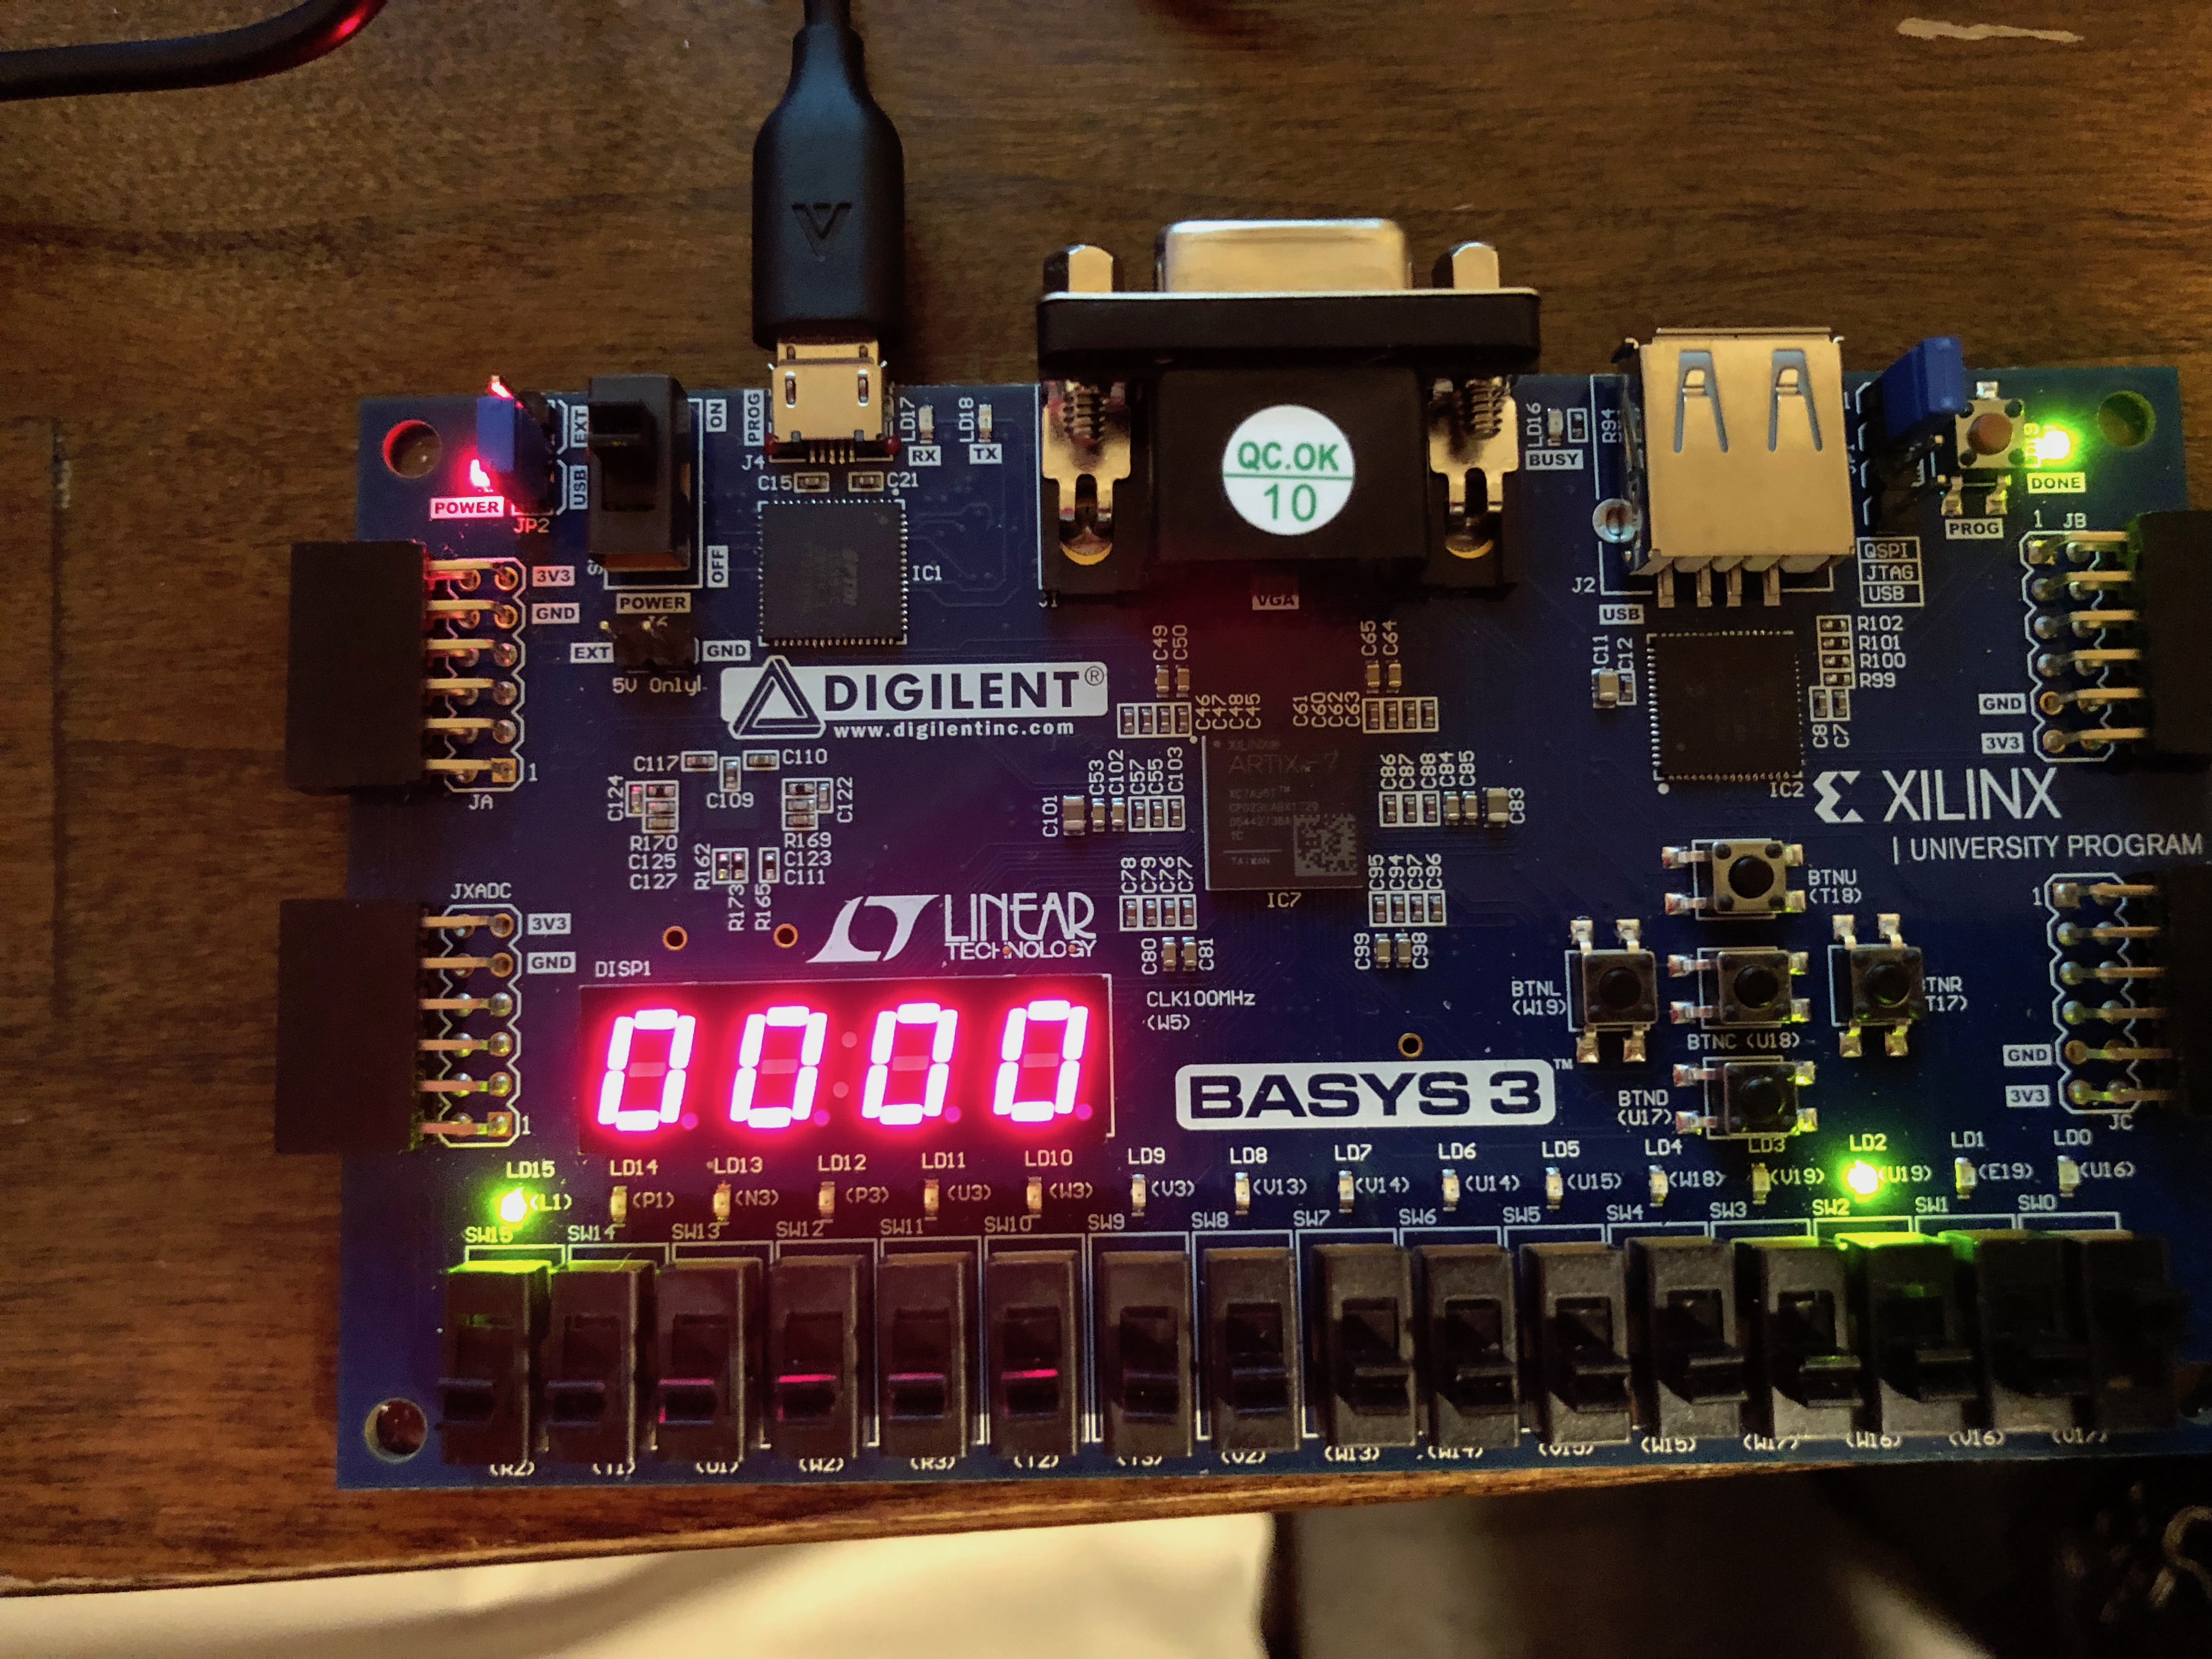
\includegraphics[width=0.5\textwidth]{./images/Part2/IMG_0579.jpg}
	\caption{\label{fig:part2img2}This image shows the state machine with an input of '1' that has progressed to State 2. In accordance with the state diagram, the output is 0.}
\end{figure}
\end{center}

\begin{center}
\begin{figure}[H]
	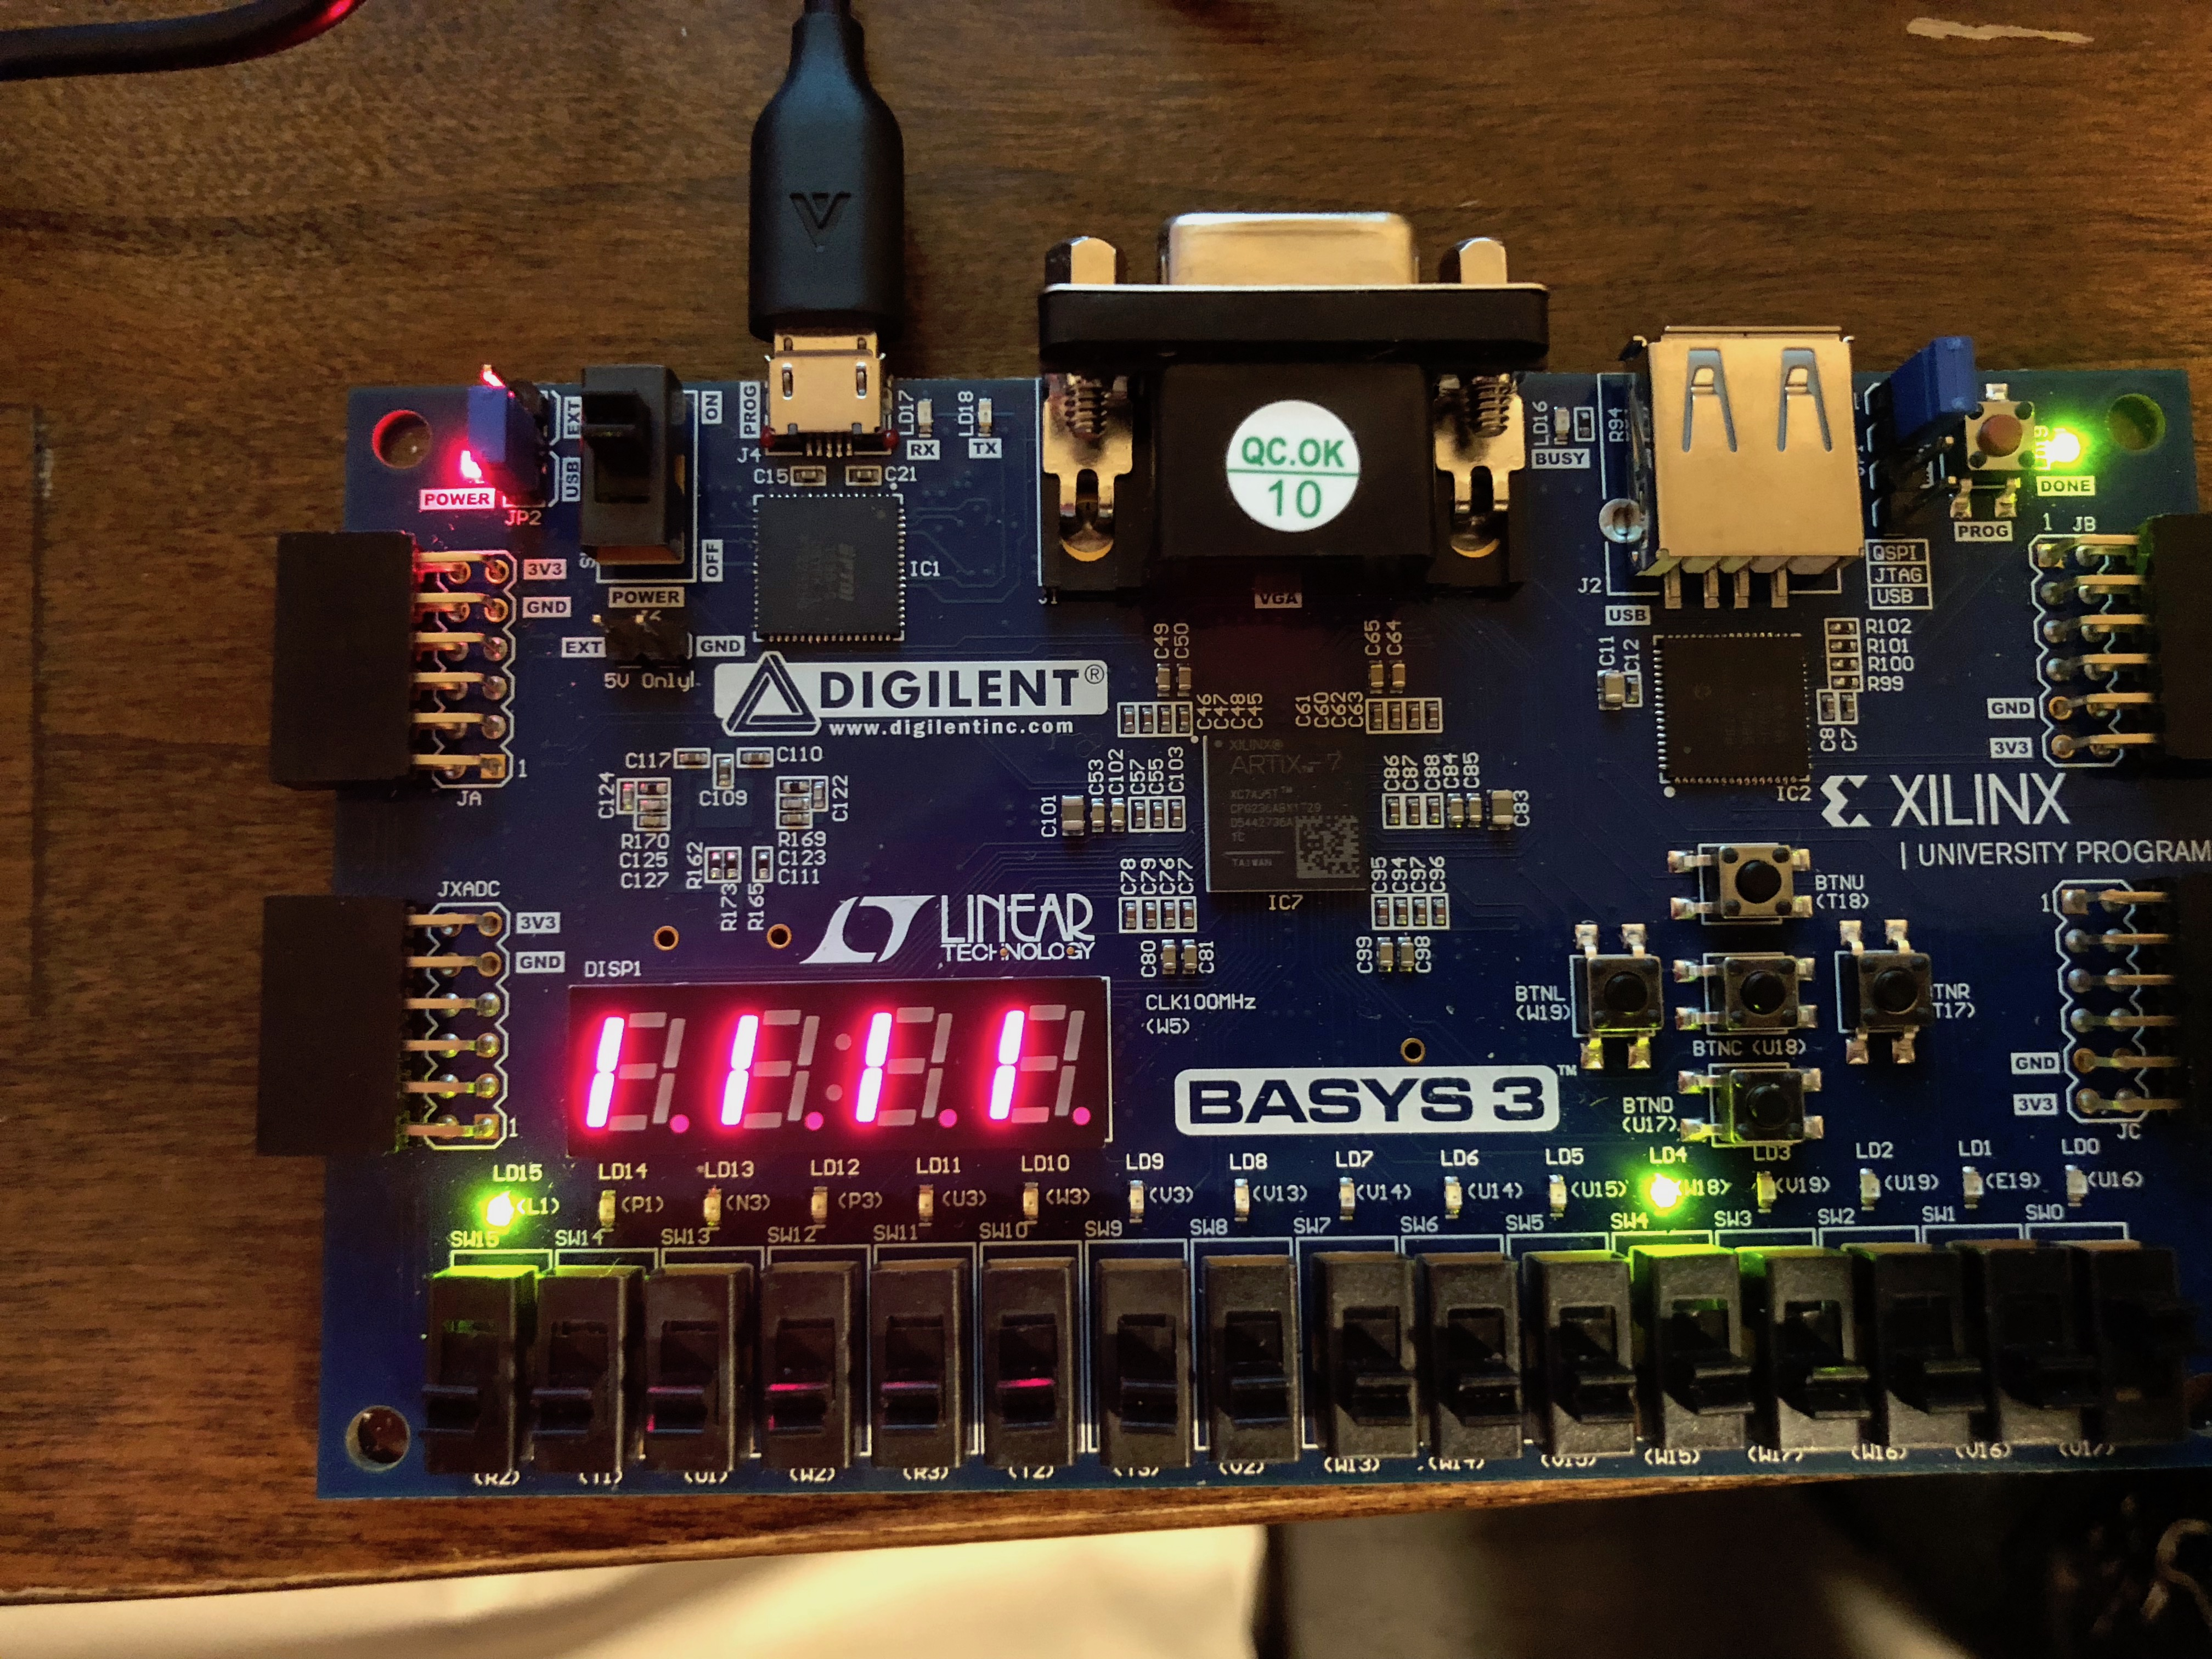
\includegraphics[width=0.5\textwidth]{./images/Part2/IMG_0580.jpg}
	\caption{\label{fig:part2img3}This image shows the state machine with a '1' input that has progressed to State 4. It is now outputting a '1' as is shown on the 7-segment display.}
\end{figure}
\end{center}

\begin{center}
\begin{figure}[H]
	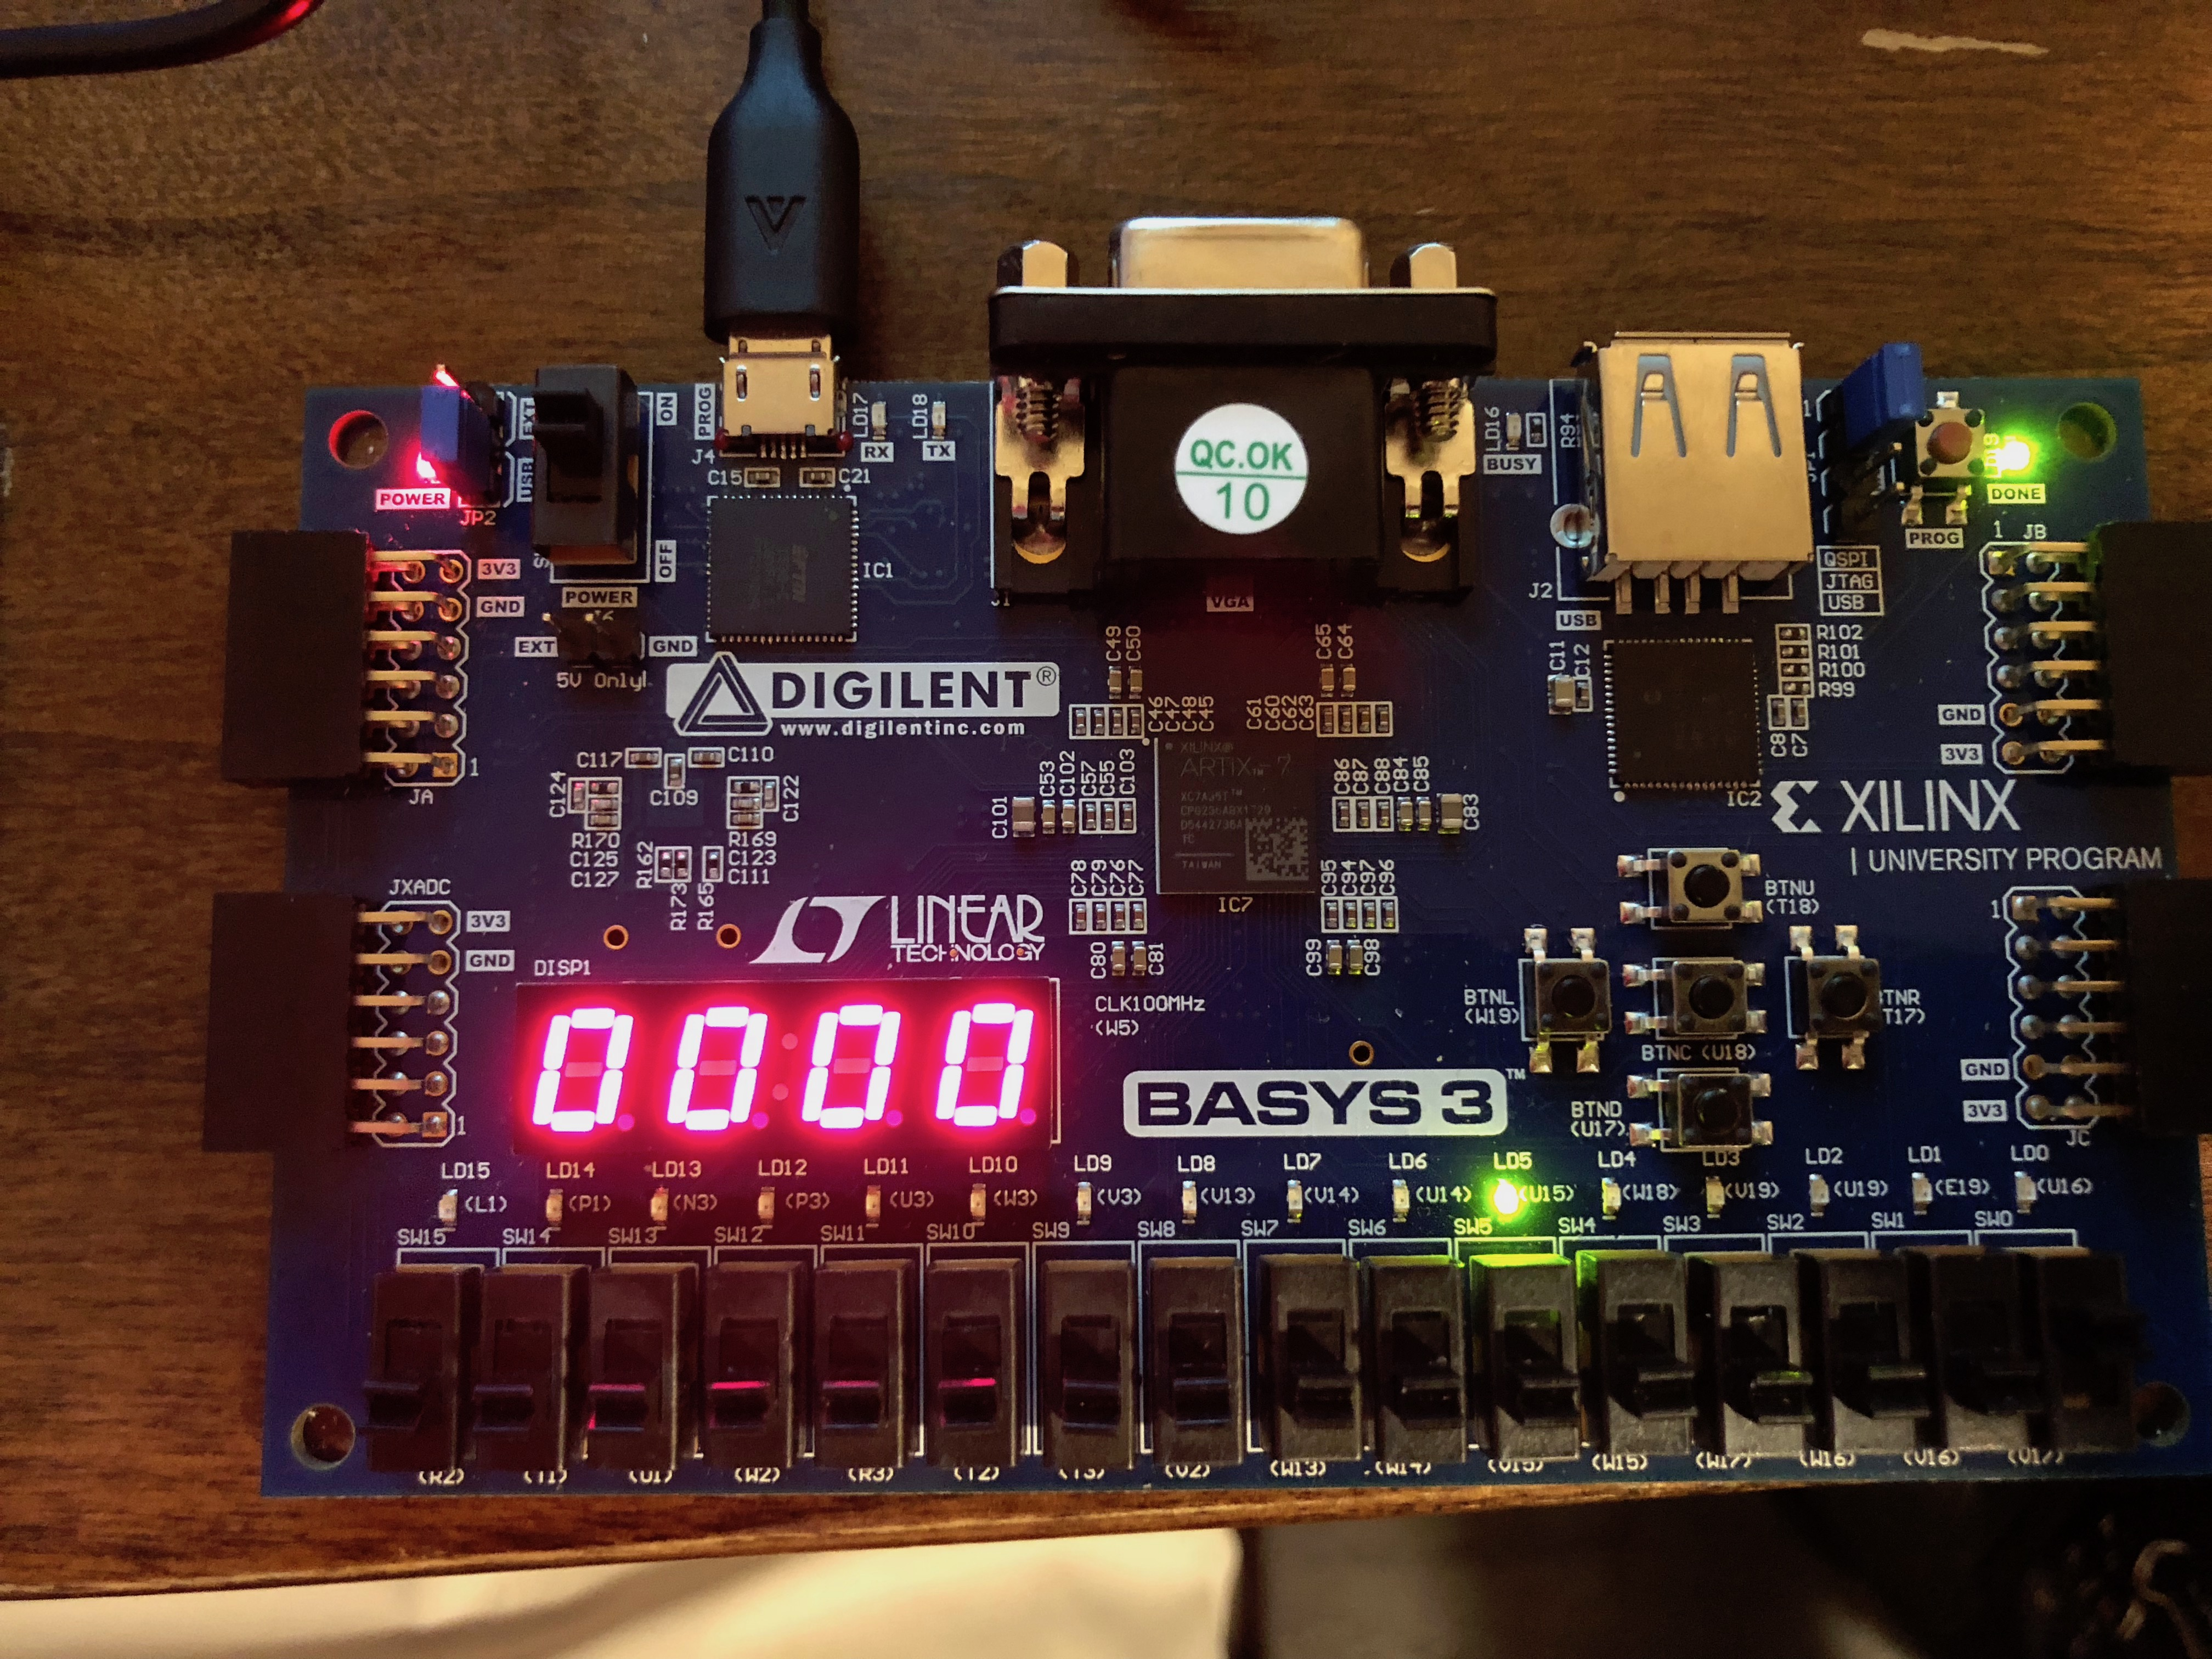
\includegraphics[width=0.5\textwidth]{./images/Part2/IMG_0581.jpg}
	\caption{\label{fig:part2img4}This image shows the state machine with an input of '1' that has progressed to State 5, and the output has returned to '0' accordingly.}
\end{figure}
\end{center}

\begin{center}
\begin{figure}[H]
	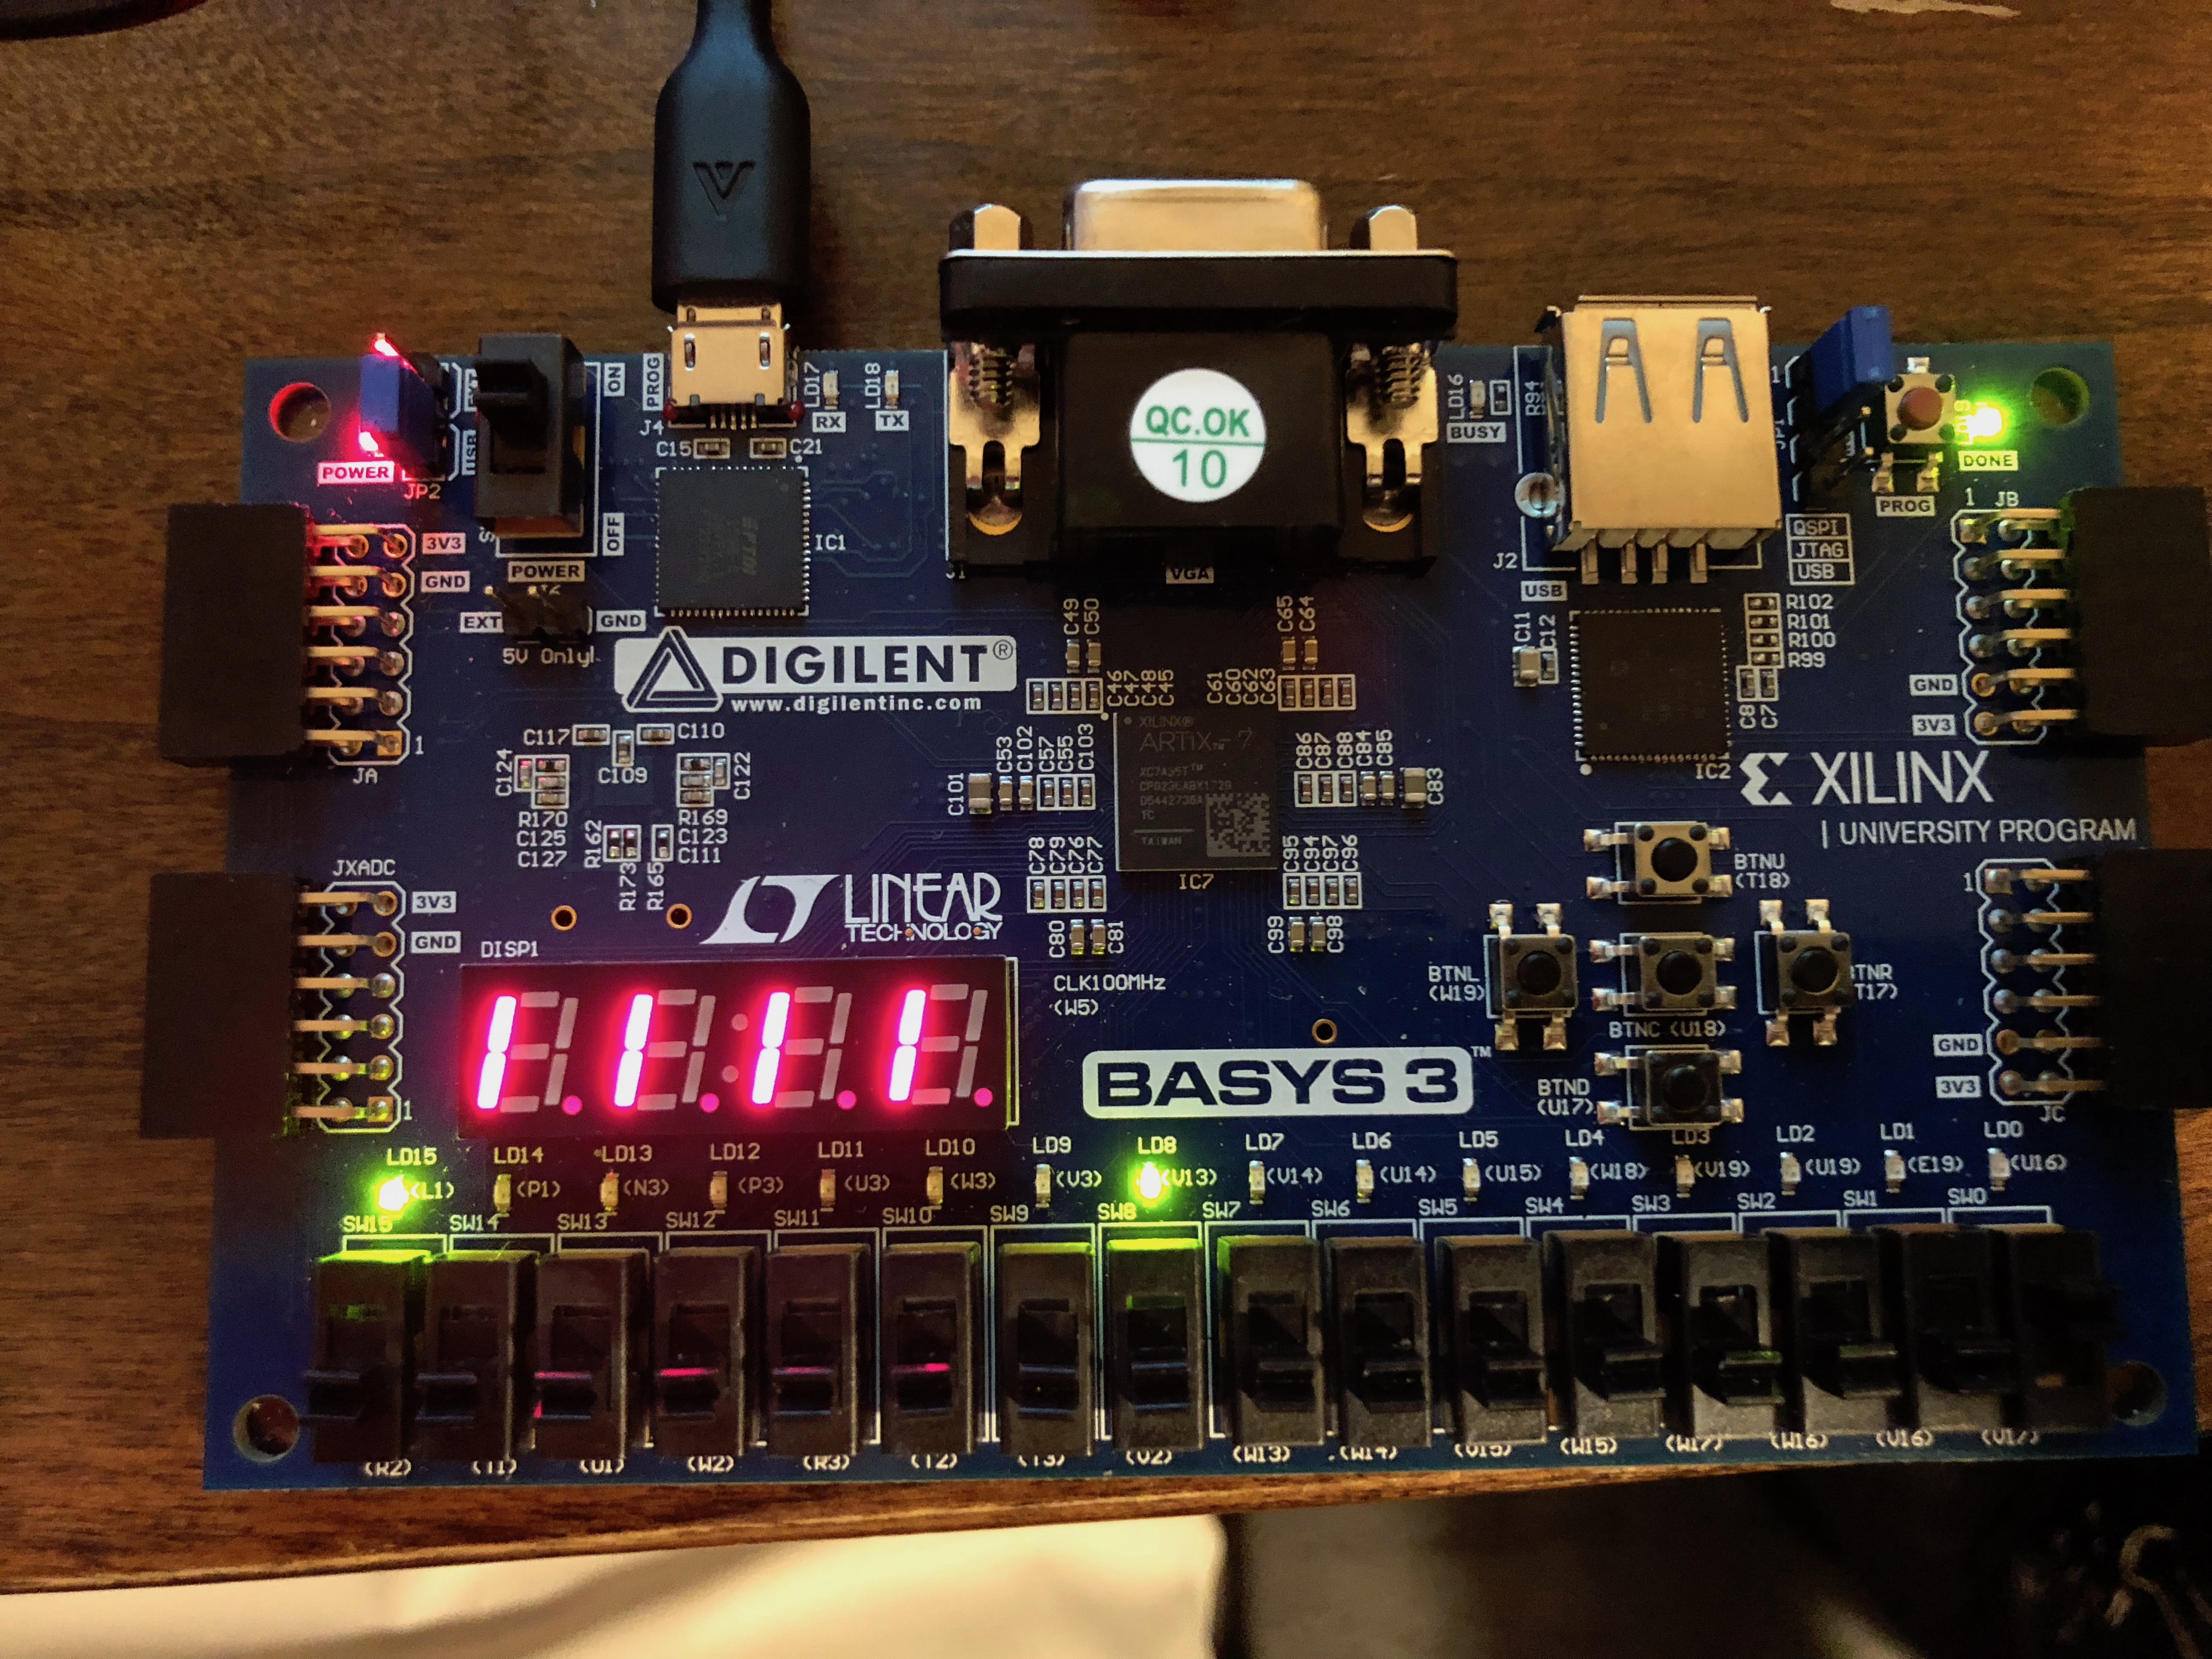
\includegraphics[width=0.5\textwidth]{./images/Part2/IMG_0582.jpg}
	\caption{\label{fig:part2img5}This image shows the state machine with an input of '1' that is in State 8. Once again, because State 8 has an output of '1', the 7-segment display shows a '1'.}
\end{figure}
\end{center}

\subsection{Problem 3}

\subsubsection{Background}
Problem 3 will use the clock divider to test a Mealy State Machine acting as a sequence detector. A Mealy State Machine provides output depending on its current state and its input. This generally lowers the amount of states required to implement a state machine. This state machine should output '1' or HIGH when either "101" or "010" is detected by the input.

\subsubsection{Design Solution}
We implemented this Mealy State Machine without overlap to detect the sequences "101" or "010". Basically, without overlap means that after detecting a sequence, the state machine returns to the original state and starts over. Therefore, if the input was "01010", the first "010" would be detected, but "10" would not trigger an output becuase the sequence has started over. The state diagram is shown in Figure ~\ref{fig:mealy_machine}. Port assignments for this design are shown in Tables ~\ref{tab:mealy_input_ports} and ~\ref{tab:_mealy_output_ports}.

\begin{center}
\begin{figure}
	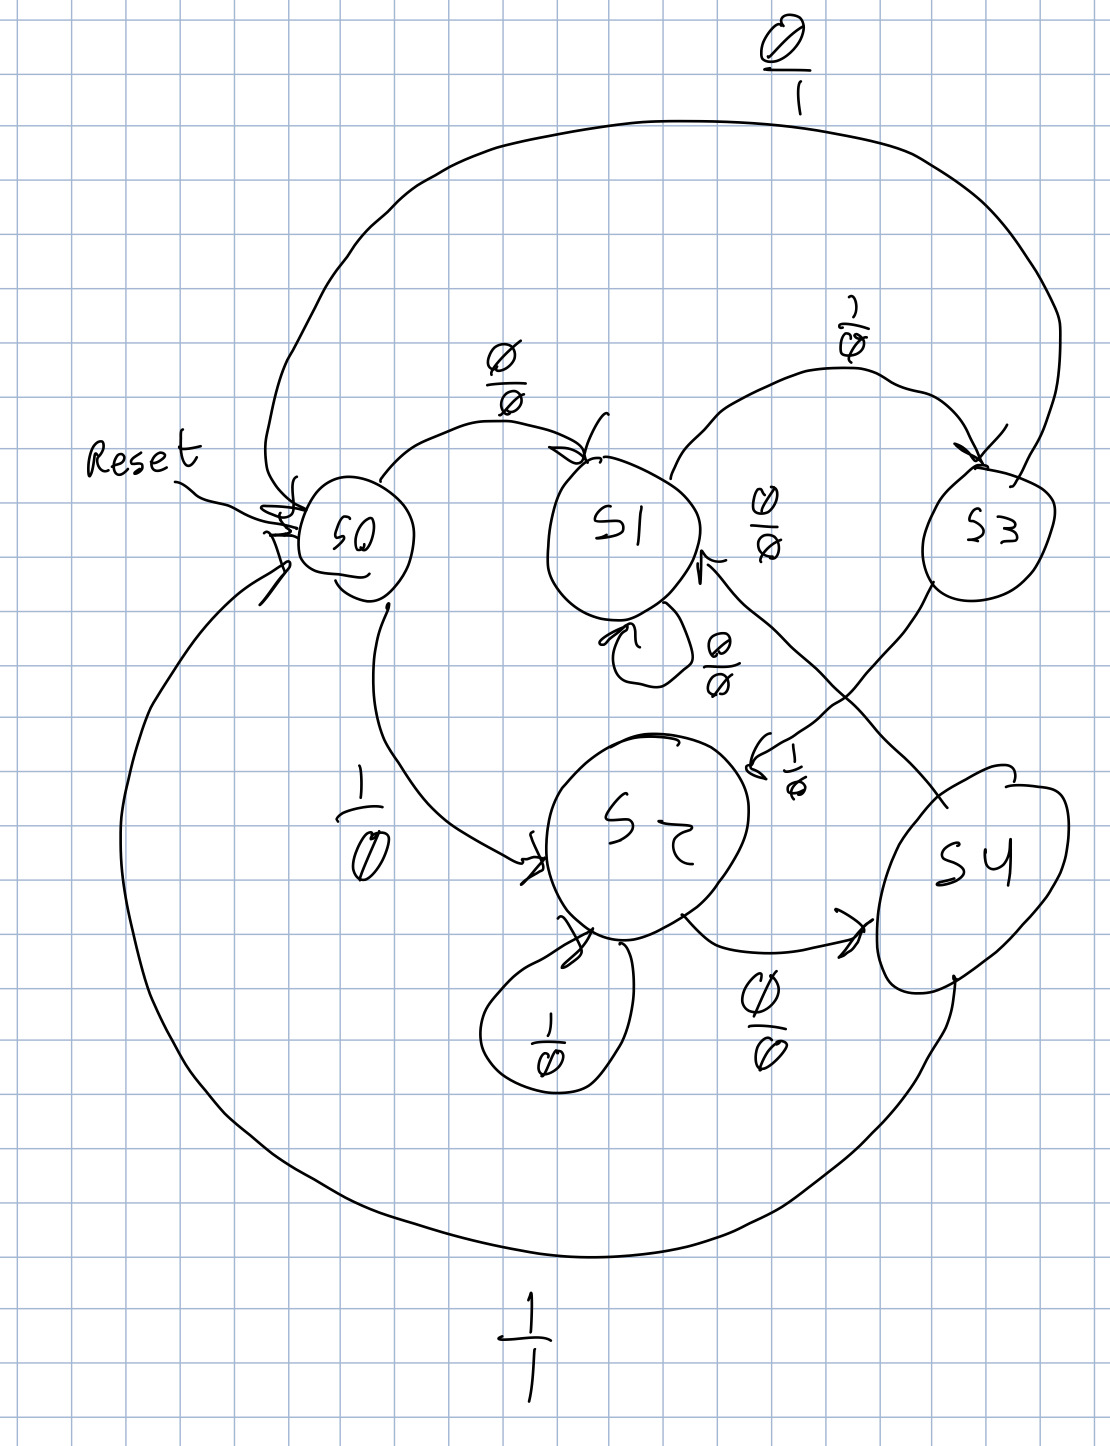
\includegraphics[width=\textwidth]{images/img2.jpg}
	\caption{\label{fig:mealy_machine}Mealy State Diagram for sequence detector.}
\end{figure}
\end{center}

\begin{table}[H]
\begin{center}
\begin{tabular}{| l | l | l |}
	\hline
	Bit & Label & Port \\ \hline
	clk & Clock & W5 \\ \hline
	clockreset & Button L & W19 \\ \hline
	reset & Button C & U18 \\ \hline
	enable & Switch 0 & V17 \\ \hline
	input & Switch 1 & U18 \\ \hline
	led0 & LED 15 & L1 \\ \hline
\end{tabular}
\caption{\label{tab:mealy_input_ports}Input port assignments for the Mealy State Machine.}
\end{center}
\end{table}

\begin{table}[H]
\begin{center}
\begin{tabular}{| l | l | l |}
	\hline
	Bit & Label & Port \\ \hline
	led0 & LED 15 & L1 \\ \hline
	state0 & LED 0 & U16 \\ \hline
	state1 & LED 1 & E19 \\ \hline
 	state2 & LED 2 & U19 \\ \hline
	state3 & LED 3 & V19 \\ \hline
	state4 & LED 4 & W18 \\ \hline
	output0 & Segment A & W7 \\ \hline
	output1 & Segment B & W6 \\ \hline
	output2 & Segment C & U8 \\ \hline
	output3 & Segment D & V8 \\ \hline
	output4 & Segment E & U5 \\ \hline
	output5 & Segment F & V5 \\ \hline
	output6 & Segment G & U7 \\ \hline
\end{tabular}
\caption{\label{tab:mealy_output_ports}Output port assignments for the Mealy State Machine.}
\end{center}
\end{table}

\subsubsection{Results}
The Mealy State Machine was able to successfully output '1' when "101" or "010" is detected. The operation of this machine is shown in Figures ~\ref{fig:part3img1} through ~\ref{fig:part3img7}.

\begin{center}
\begin{figure}[H]
	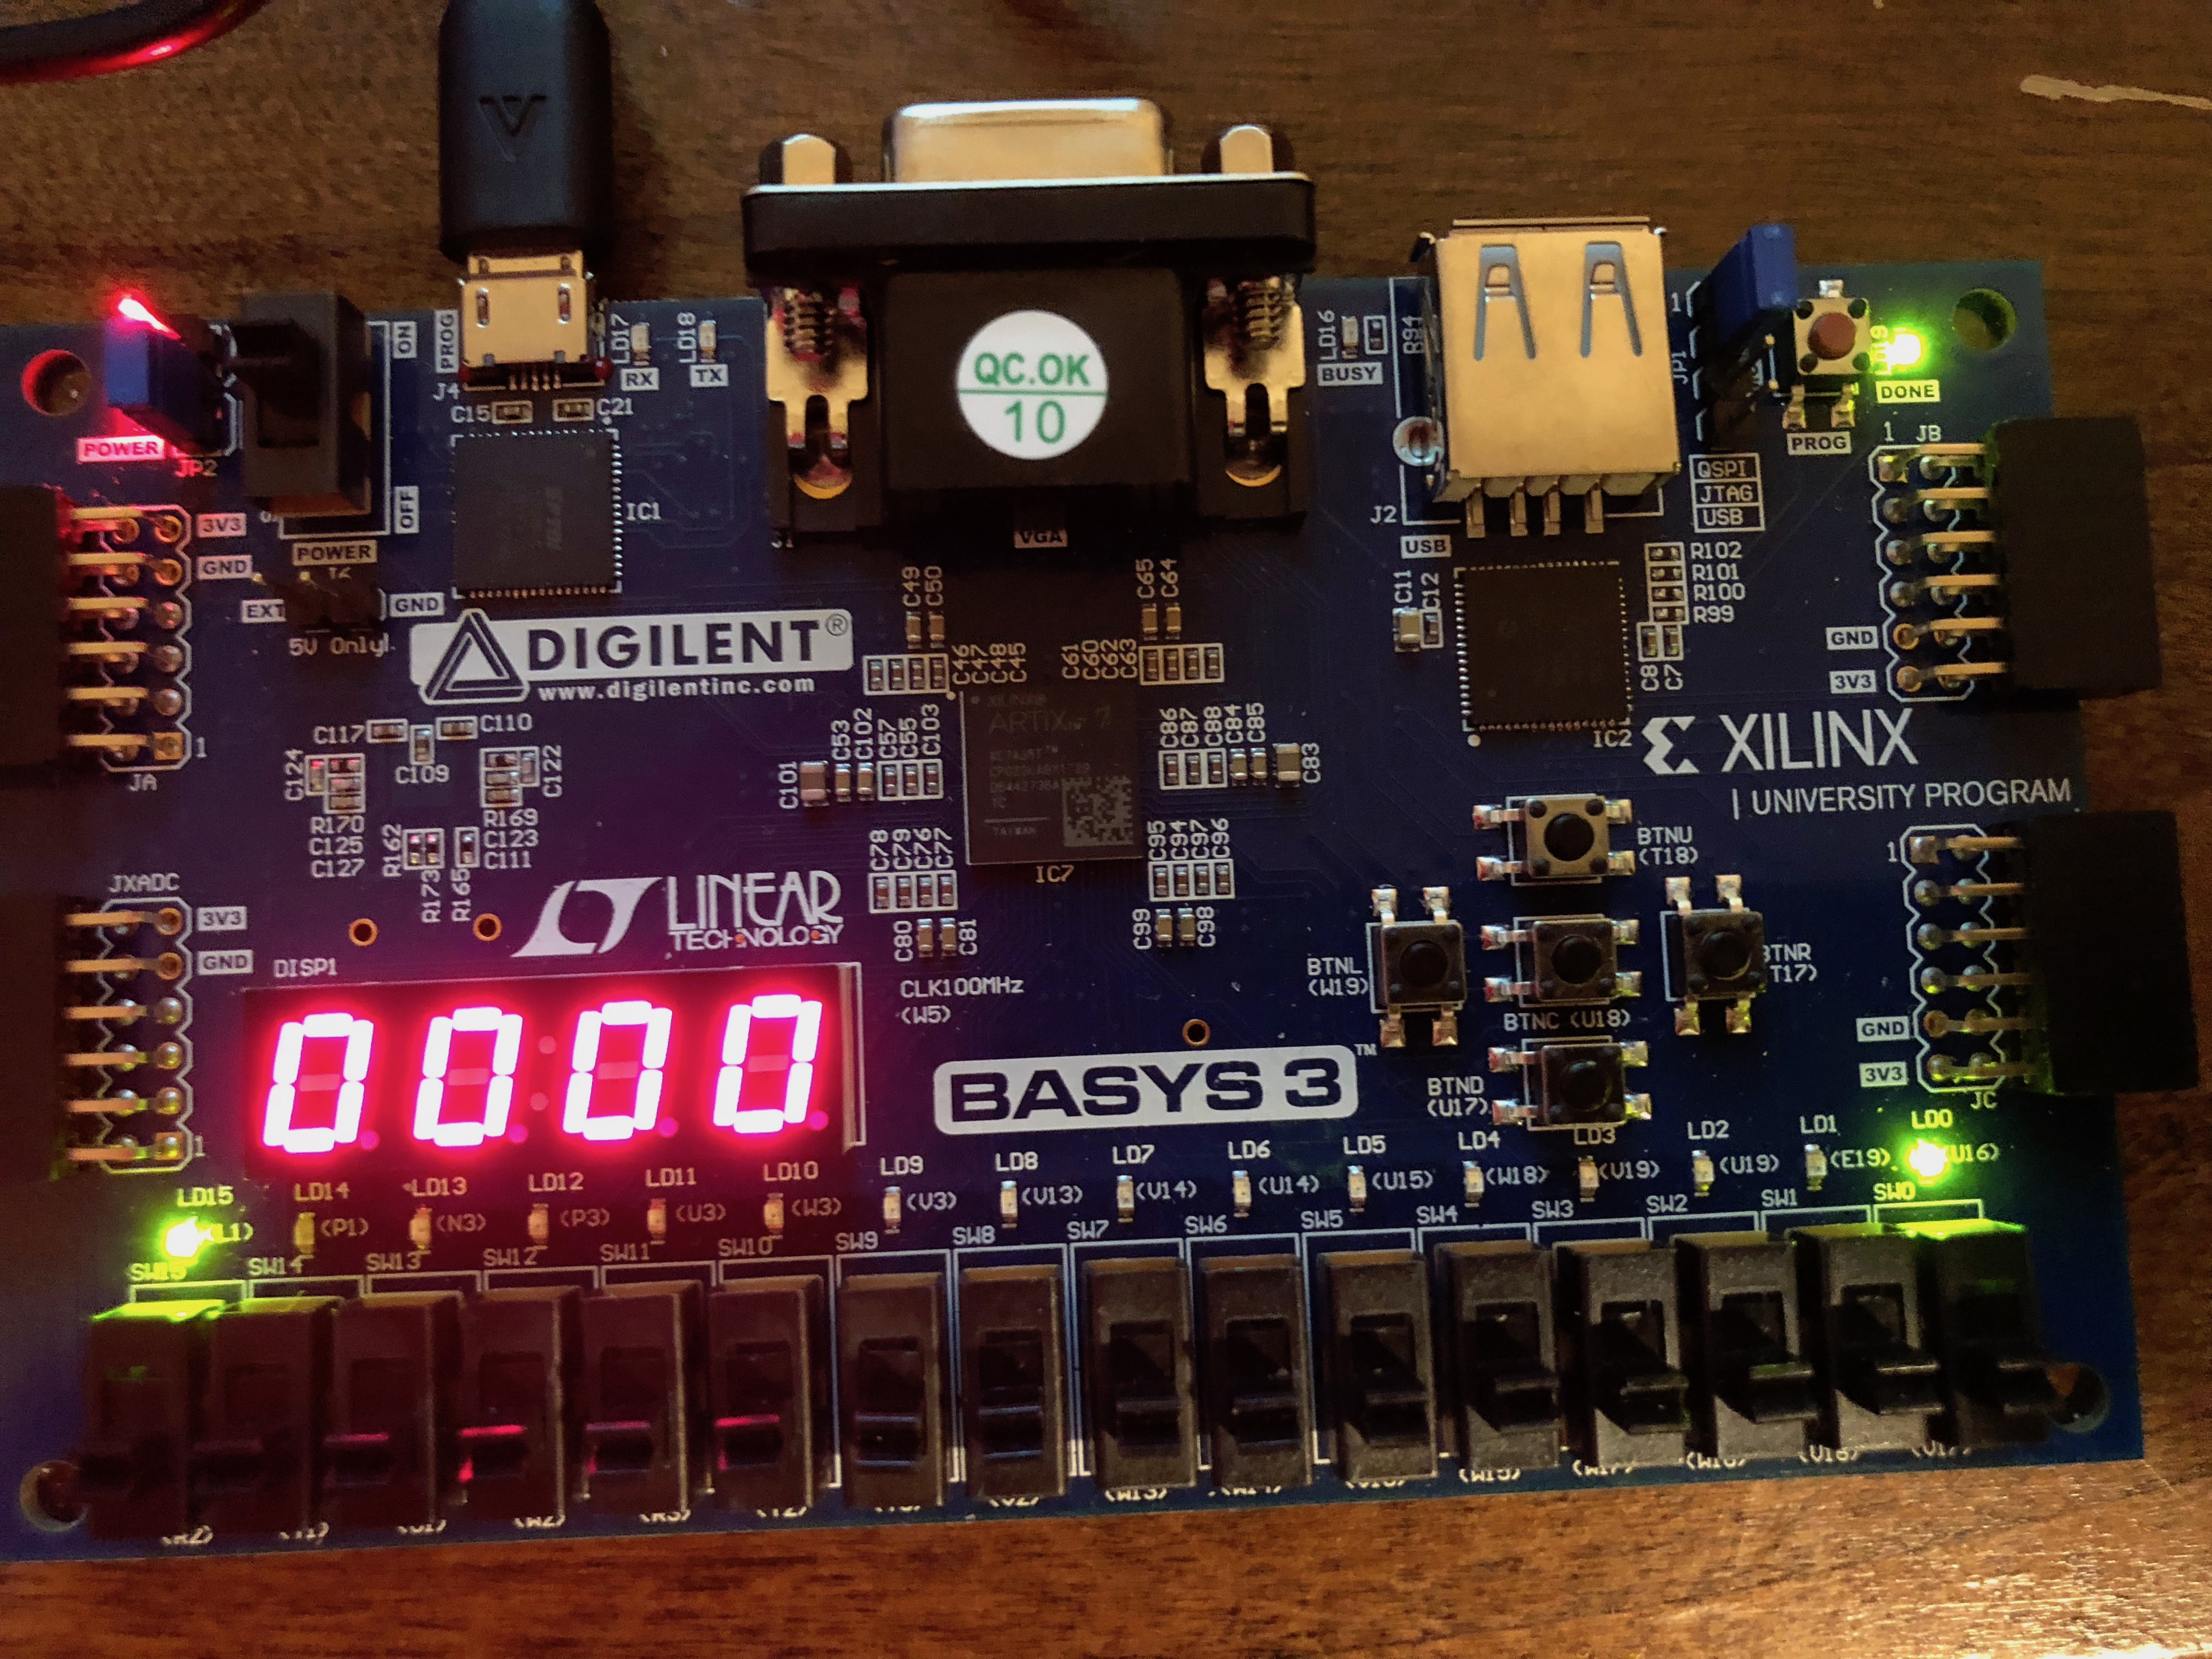
\includegraphics[width=0.5\textwidth]{./images/Part3/IMG_0583.jpg}
	\caption{\label{fig:part3img1}This image shows the state machine with an input of '0' that is currently disabled. Therefore, it is remaining in State 0 regardless of input.}
\end{figure}
\end{center}

\begin{center}
\begin{figure}[H]
	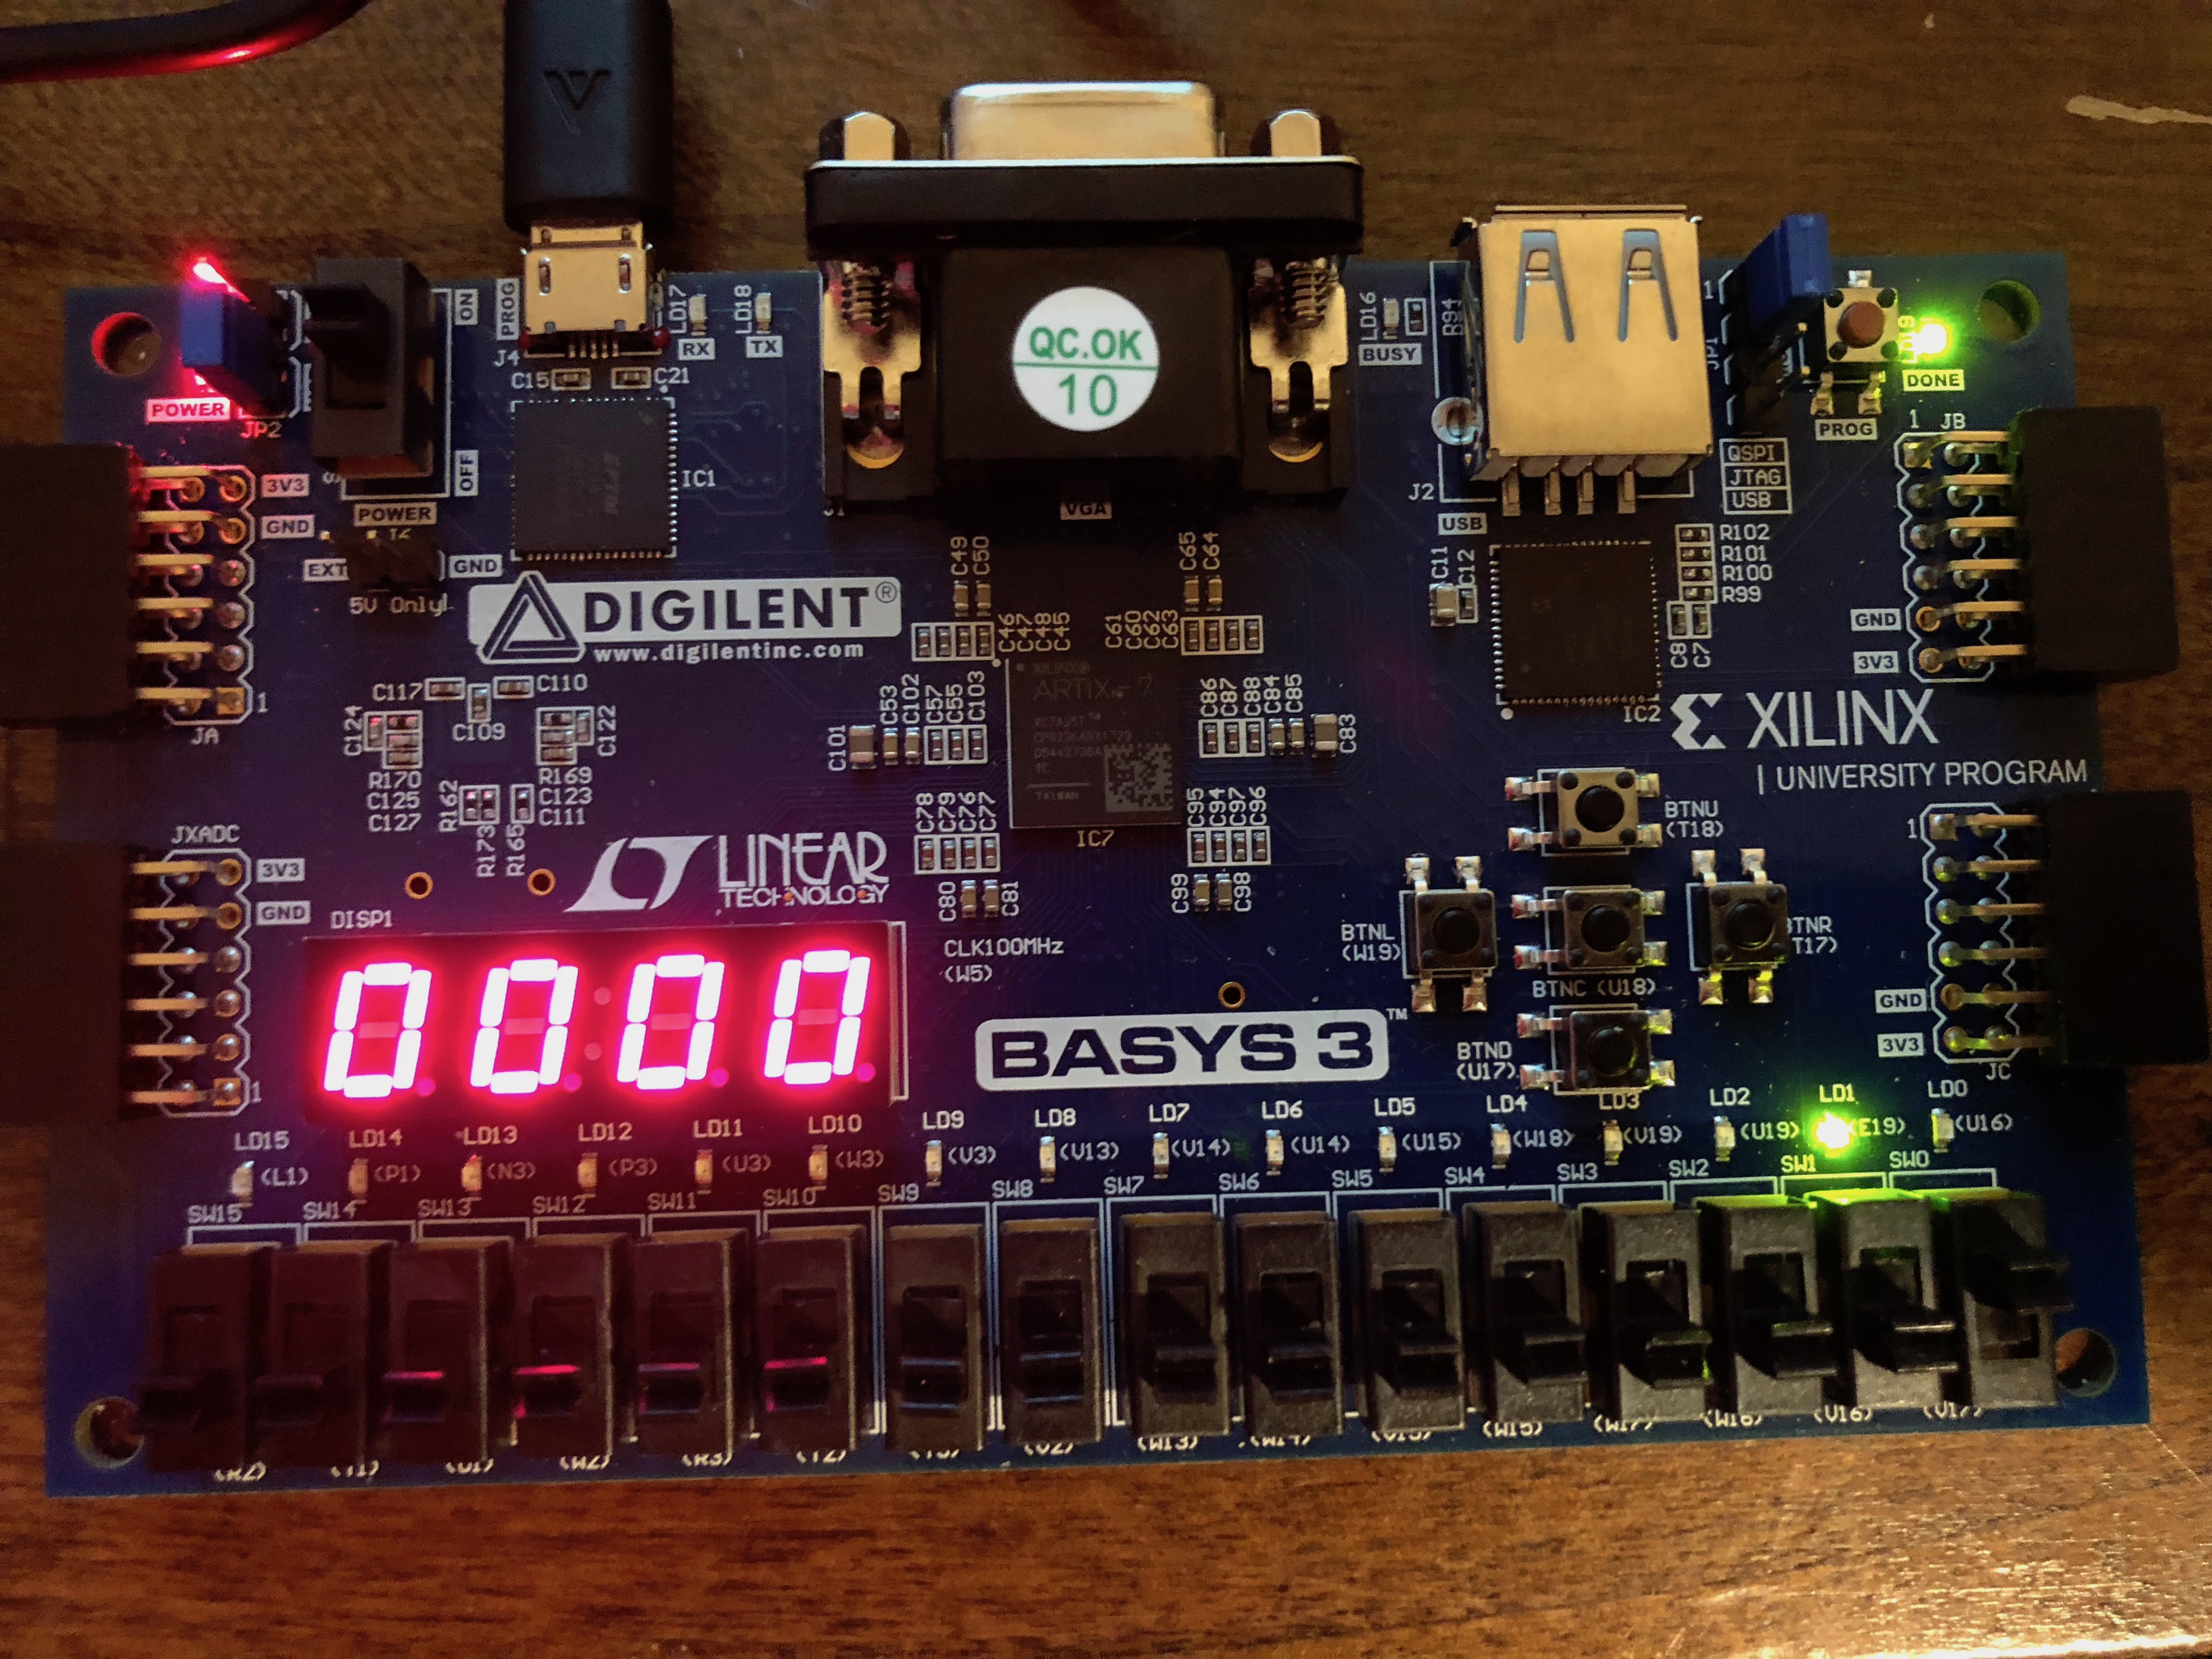
\includegraphics[width=0.5\textwidth]{./images/Part3/IMG_0584.jpg}
	\caption{\label{fig:part3img2}This image shows the state machine that is enabled, after receiving an input of '0'. Therefore, it has progressed to State 1 and will remain there per the state diagram until it detects an input of '1'.}
\end{figure}
\end{center}

\begin{center}
\begin{figure}[H]
	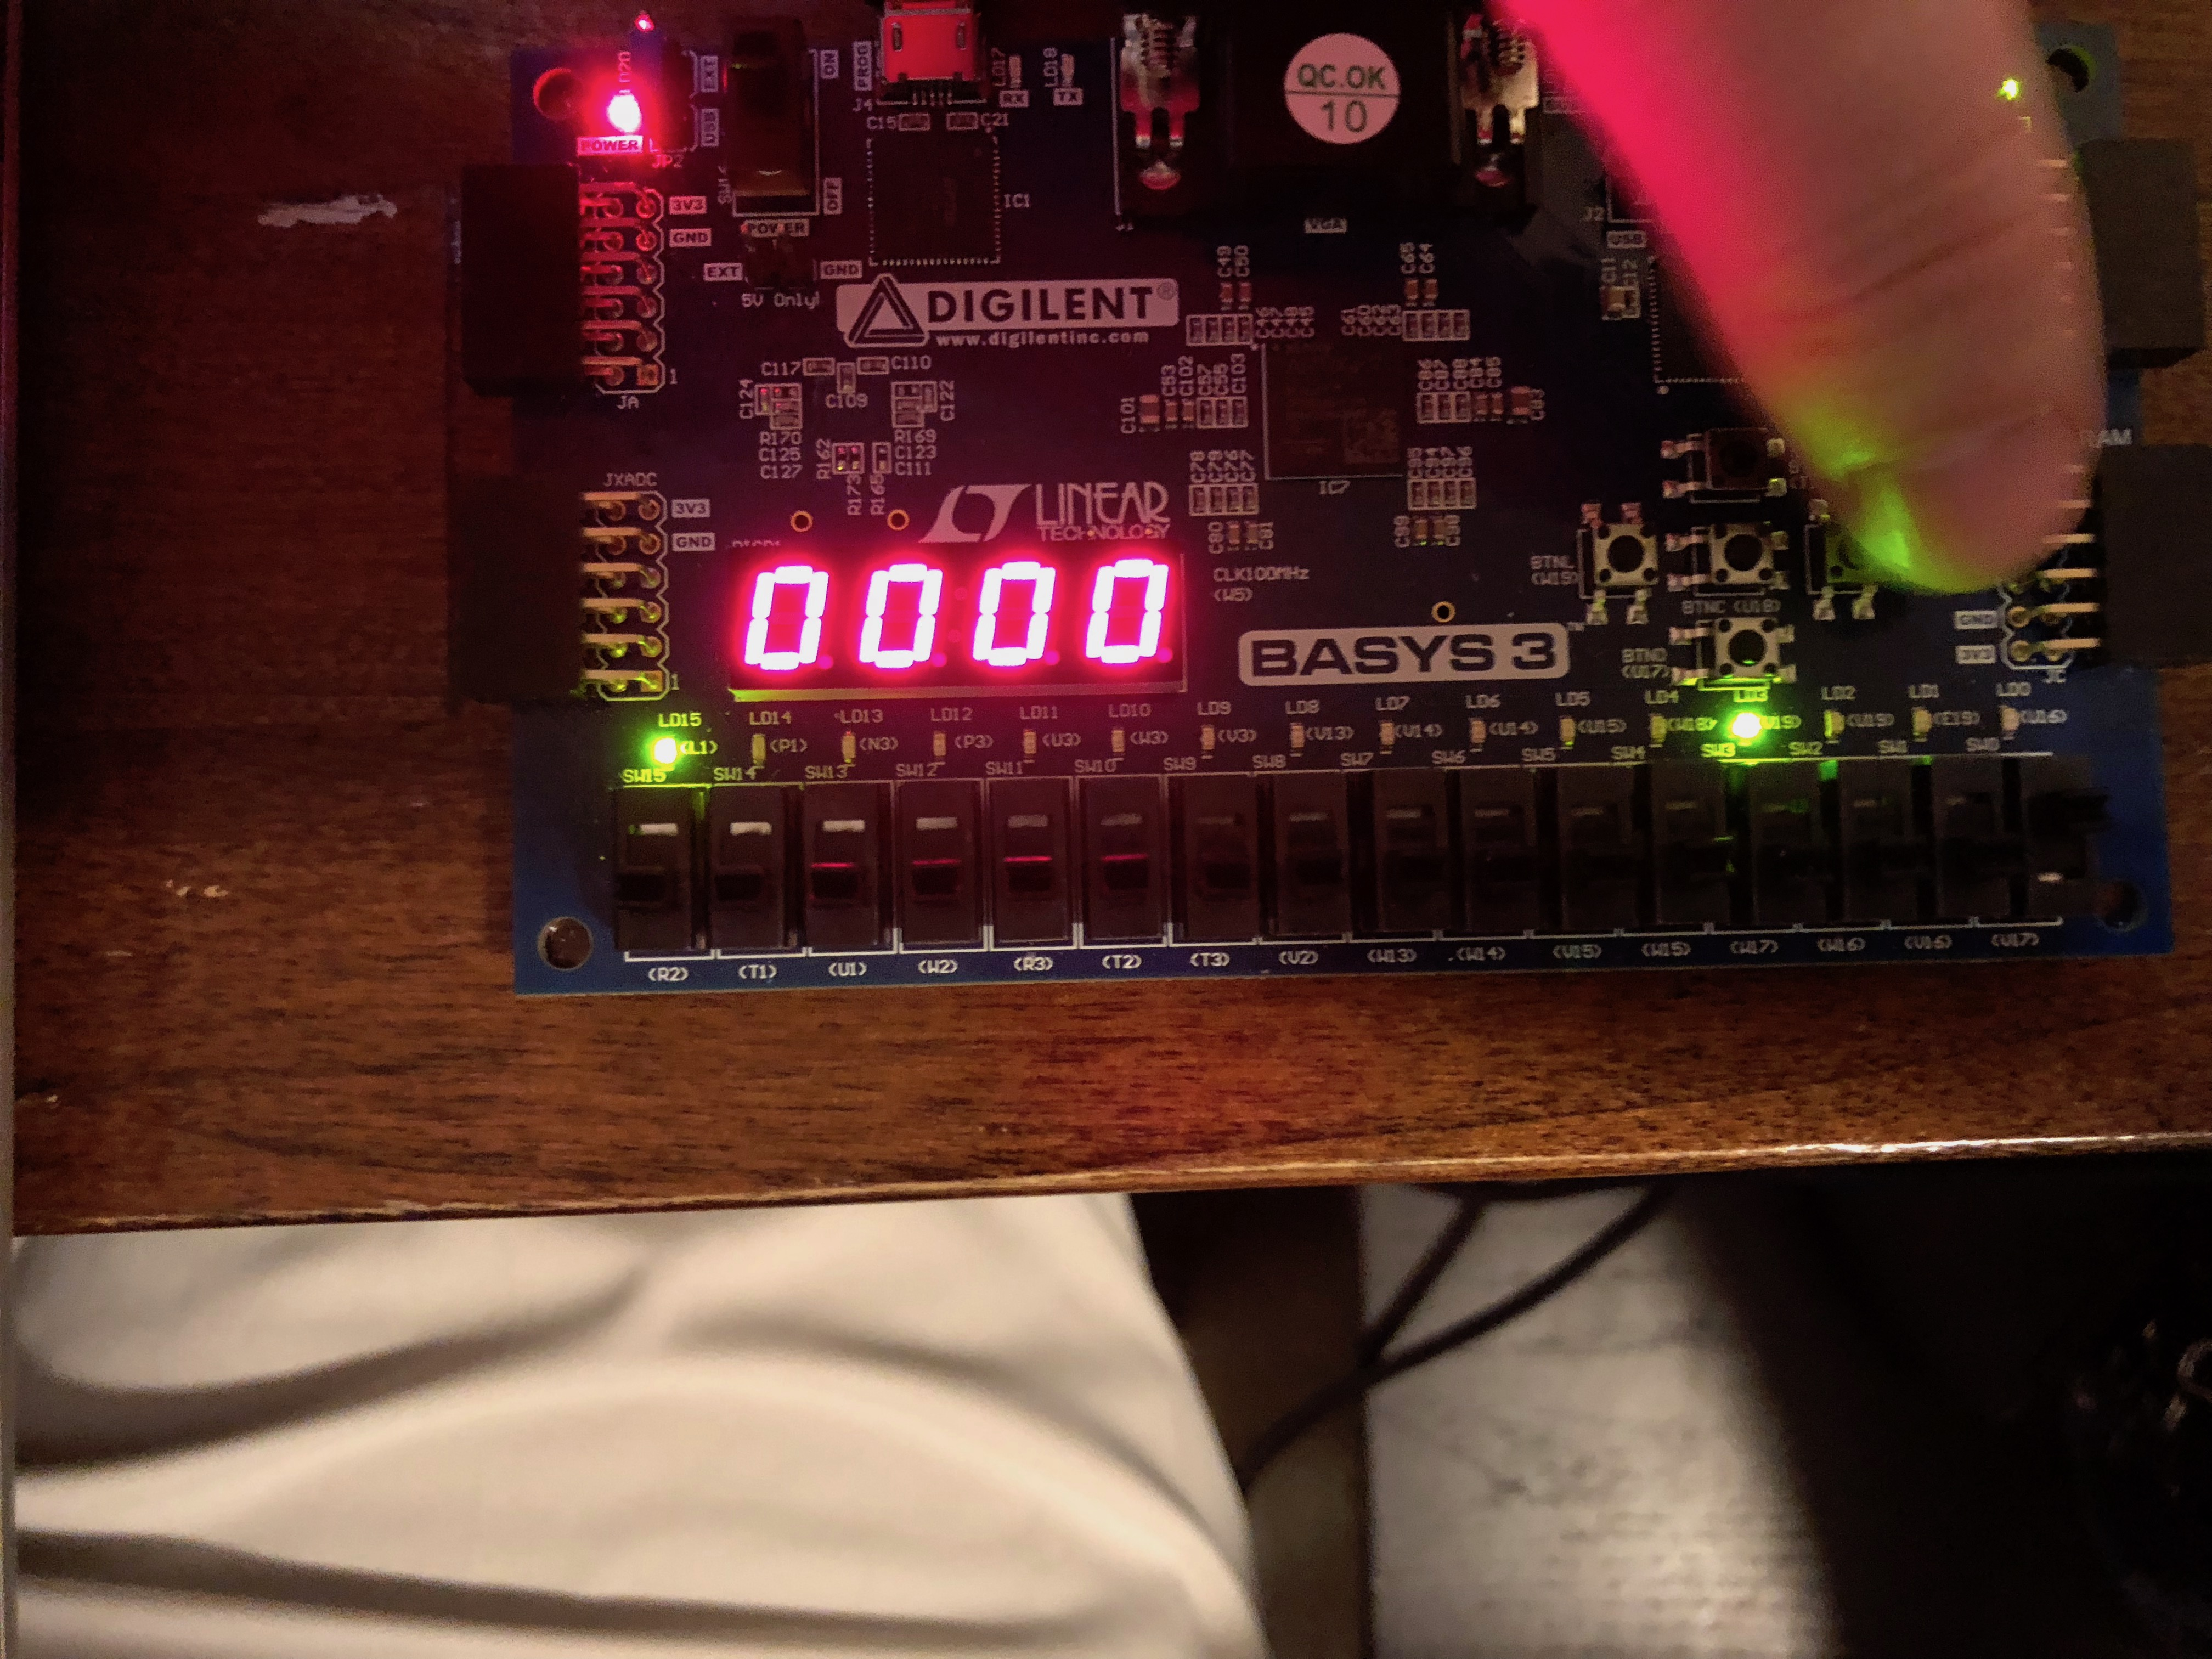
\includegraphics[width=0.5\textwidth]{./images/Part3/IMG_0585.jpg}
	\caption{\label{fig:part3img3}This image shows the state machine after receiving an input of '1' in State 1. It has progressed to State 3.}
\end{figure}
\end{center}

\begin{center}
\begin{figure}[H]
	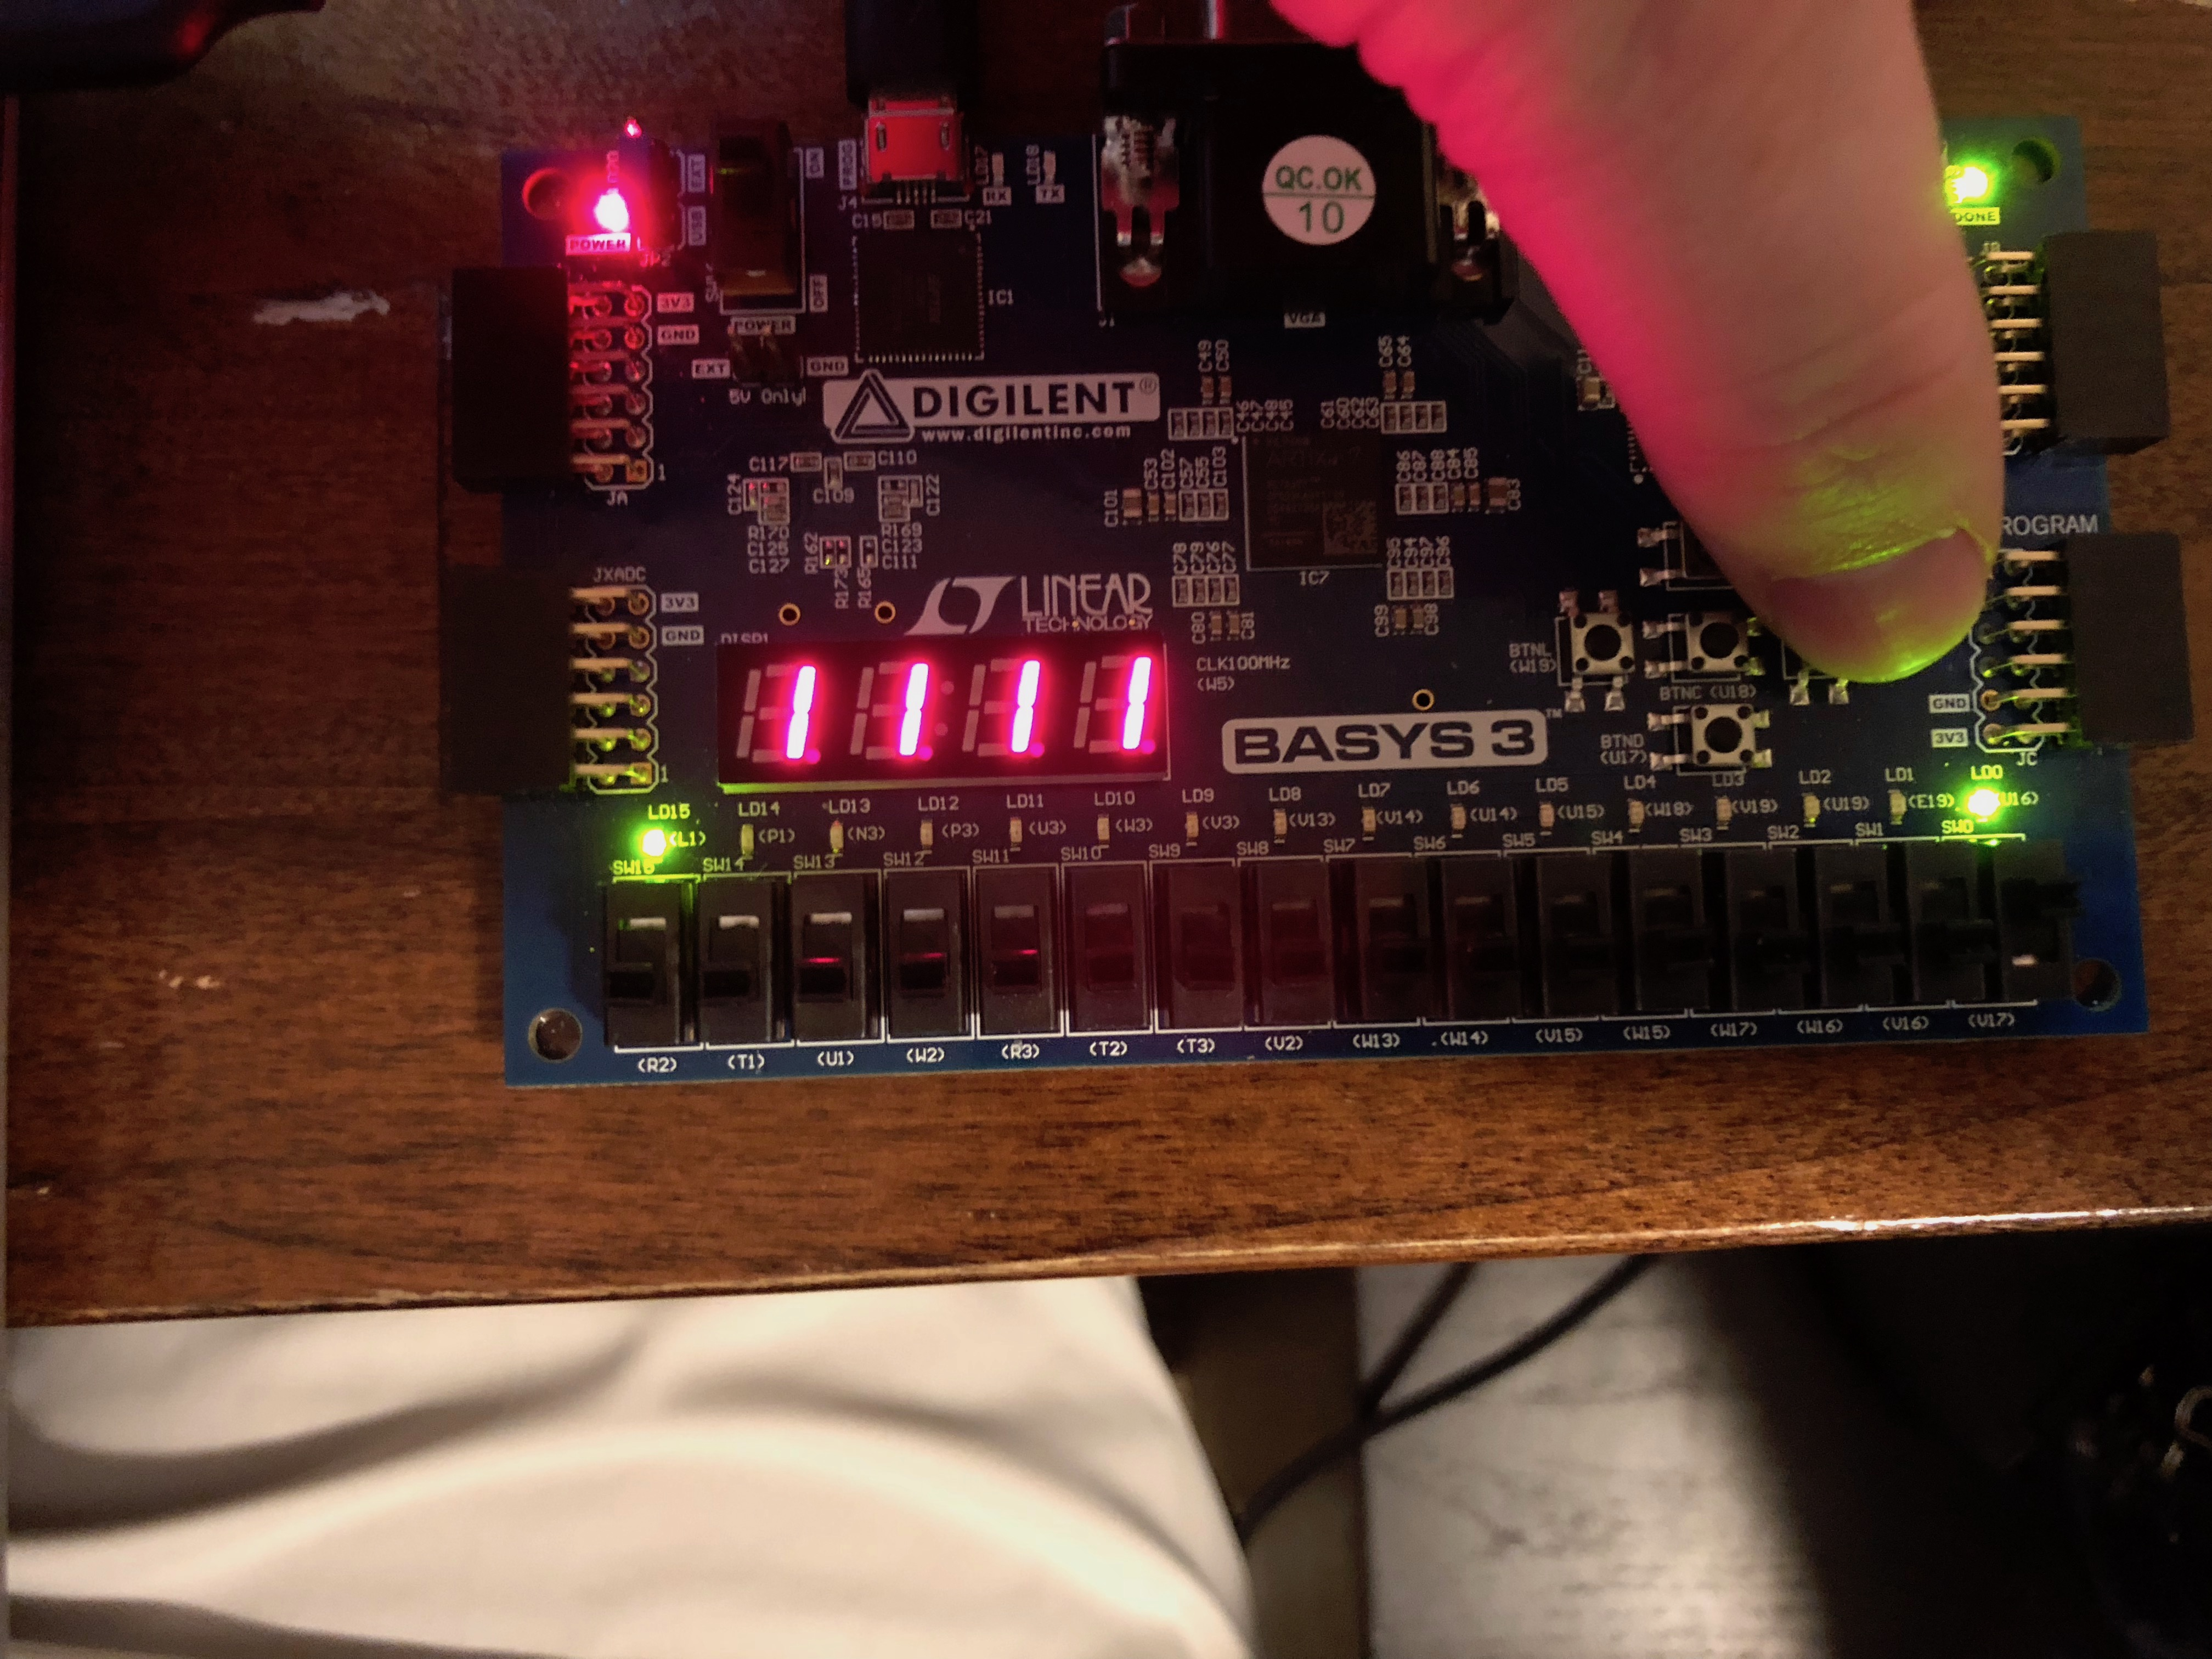
\includegraphics[width=0.5\textwidth]{./images/Part3/IMG_0586.jpg}
	\caption{\label{fig:part3img4}This image shows the state machine after receiving an input of '0' in State 3, which returns it to State 0 while outputting '1'.}
\end{figure}
\end{center}

\begin{center}
\begin{figure}[H]
	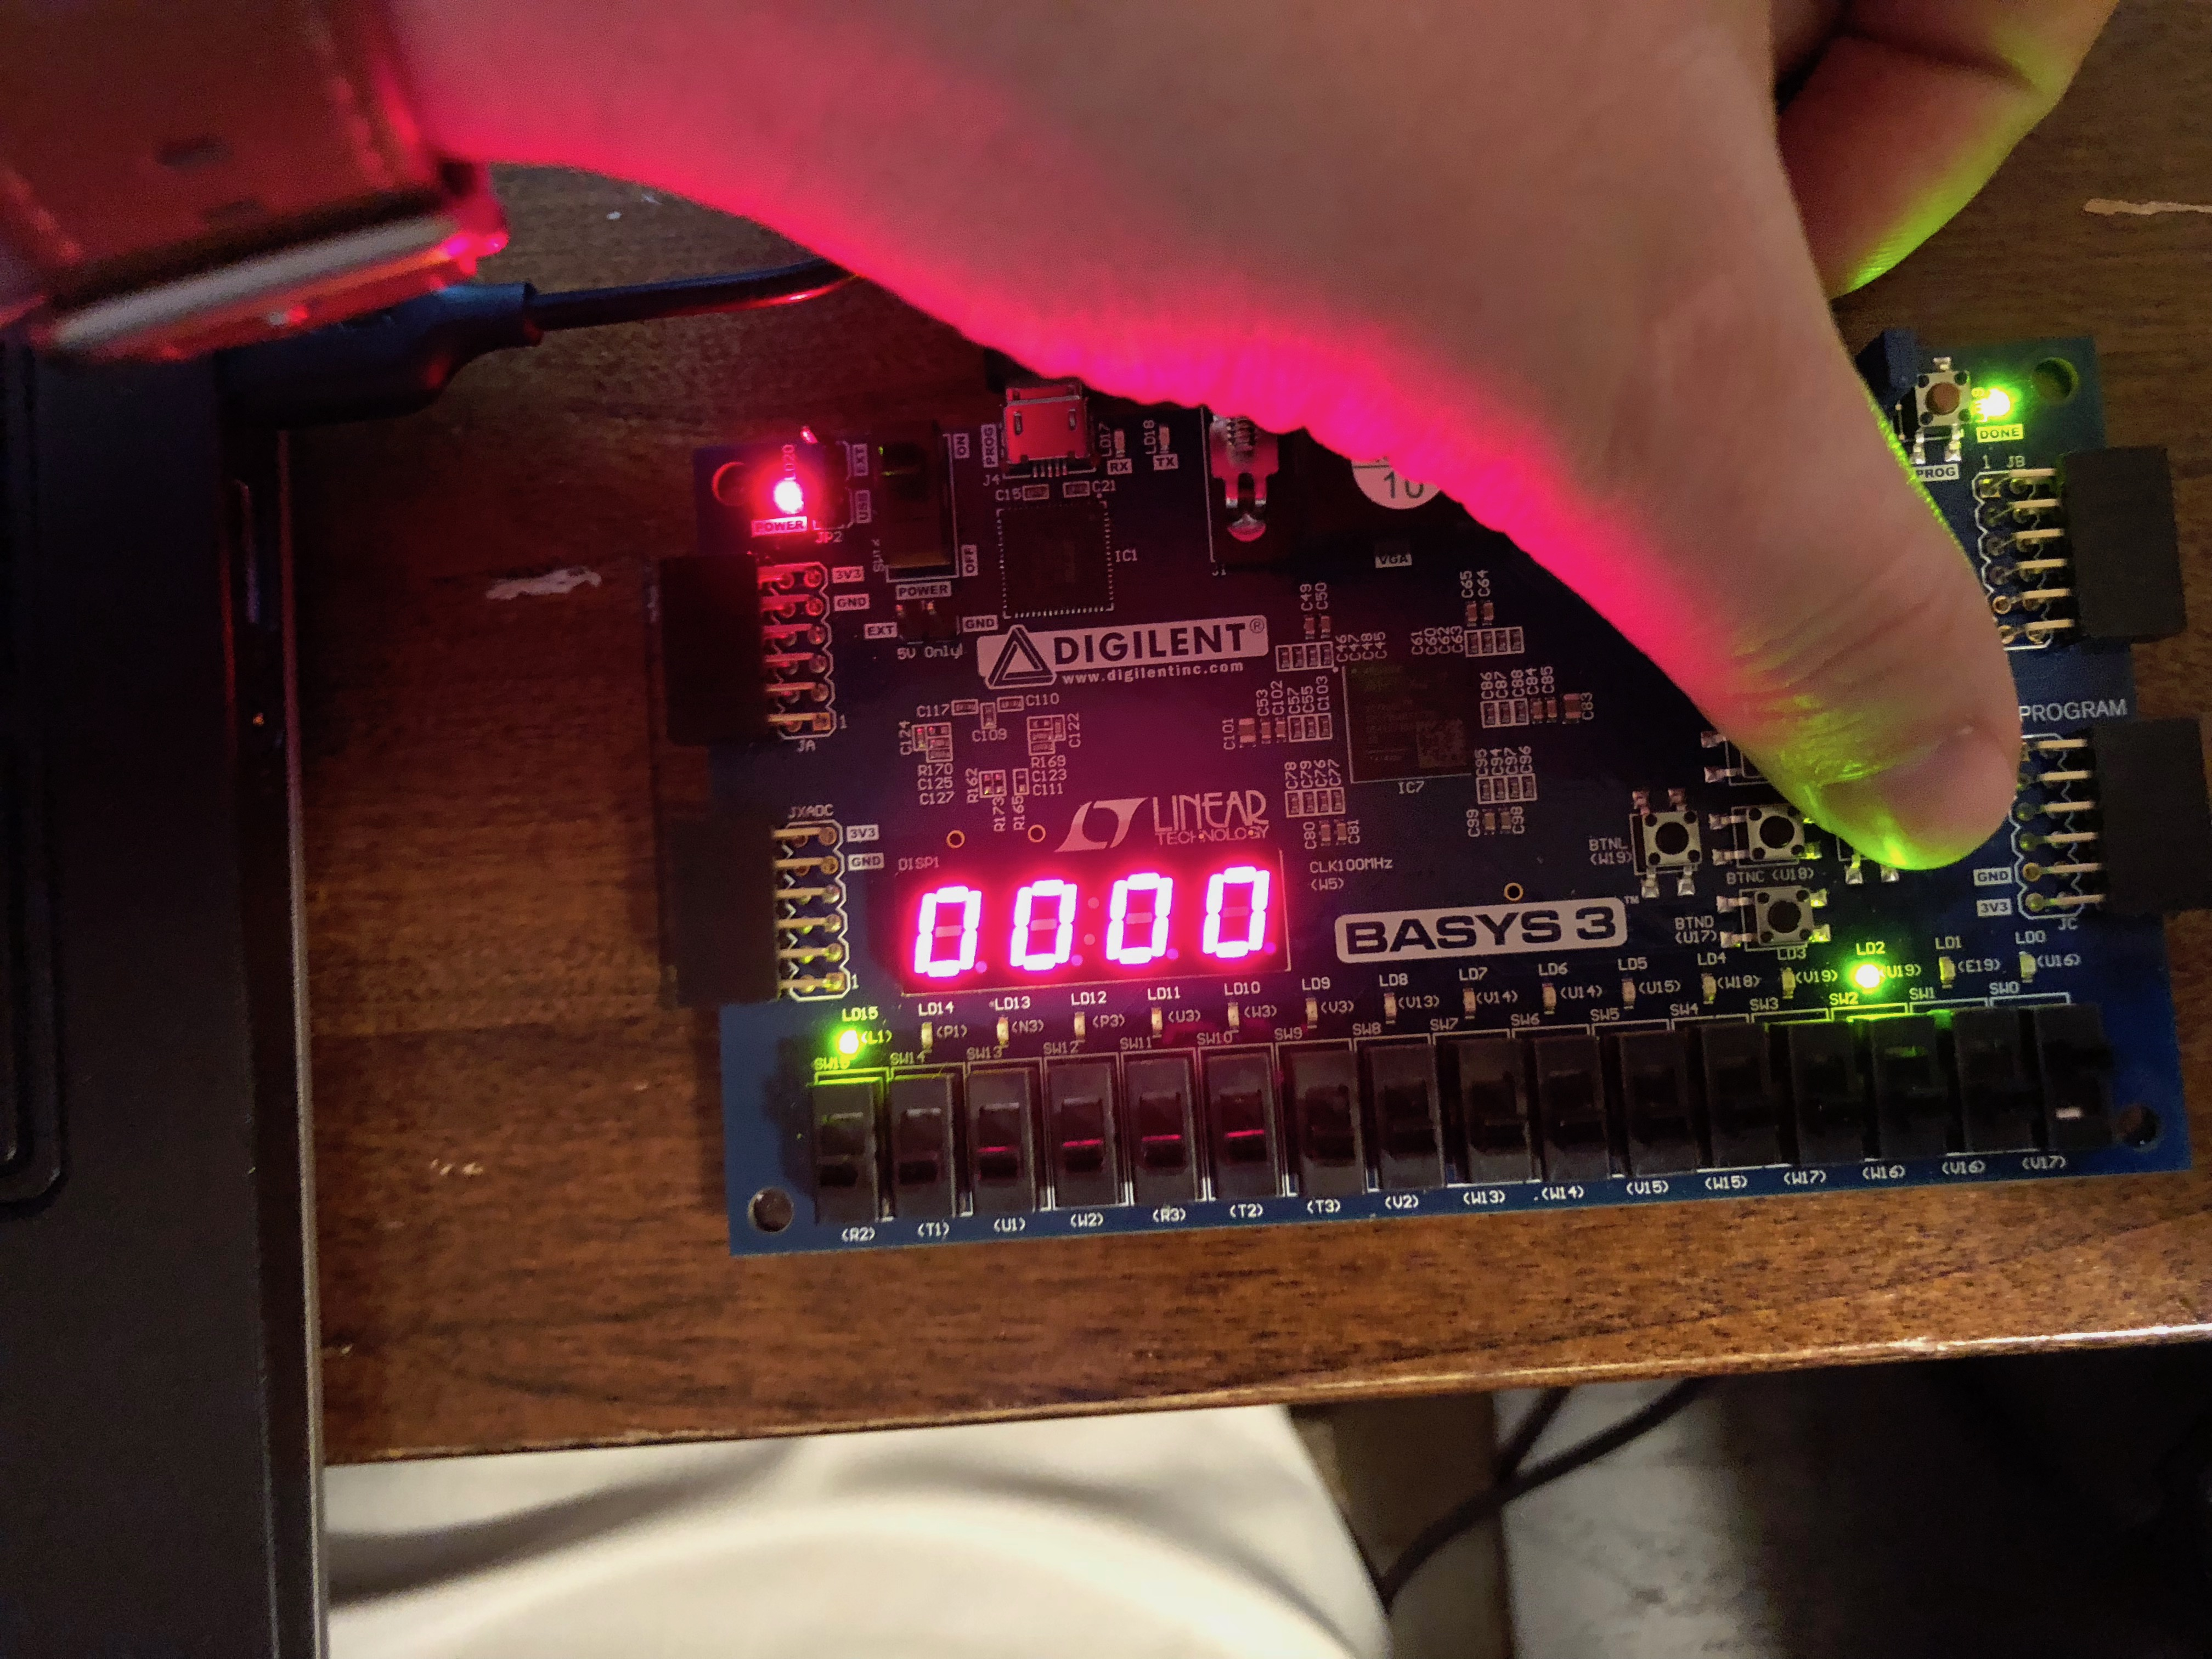
\includegraphics[width=0.5\textwidth]{./images/Part3/IMG_0587.jpg}
	\caption{\label{fig:part3img5}This image shows the state machine after receiving input '1' from State 0. Therefore, it has progressed to State 2.}
\end{figure}
\end{center}

\begin{center}
\begin{figure}[H]
	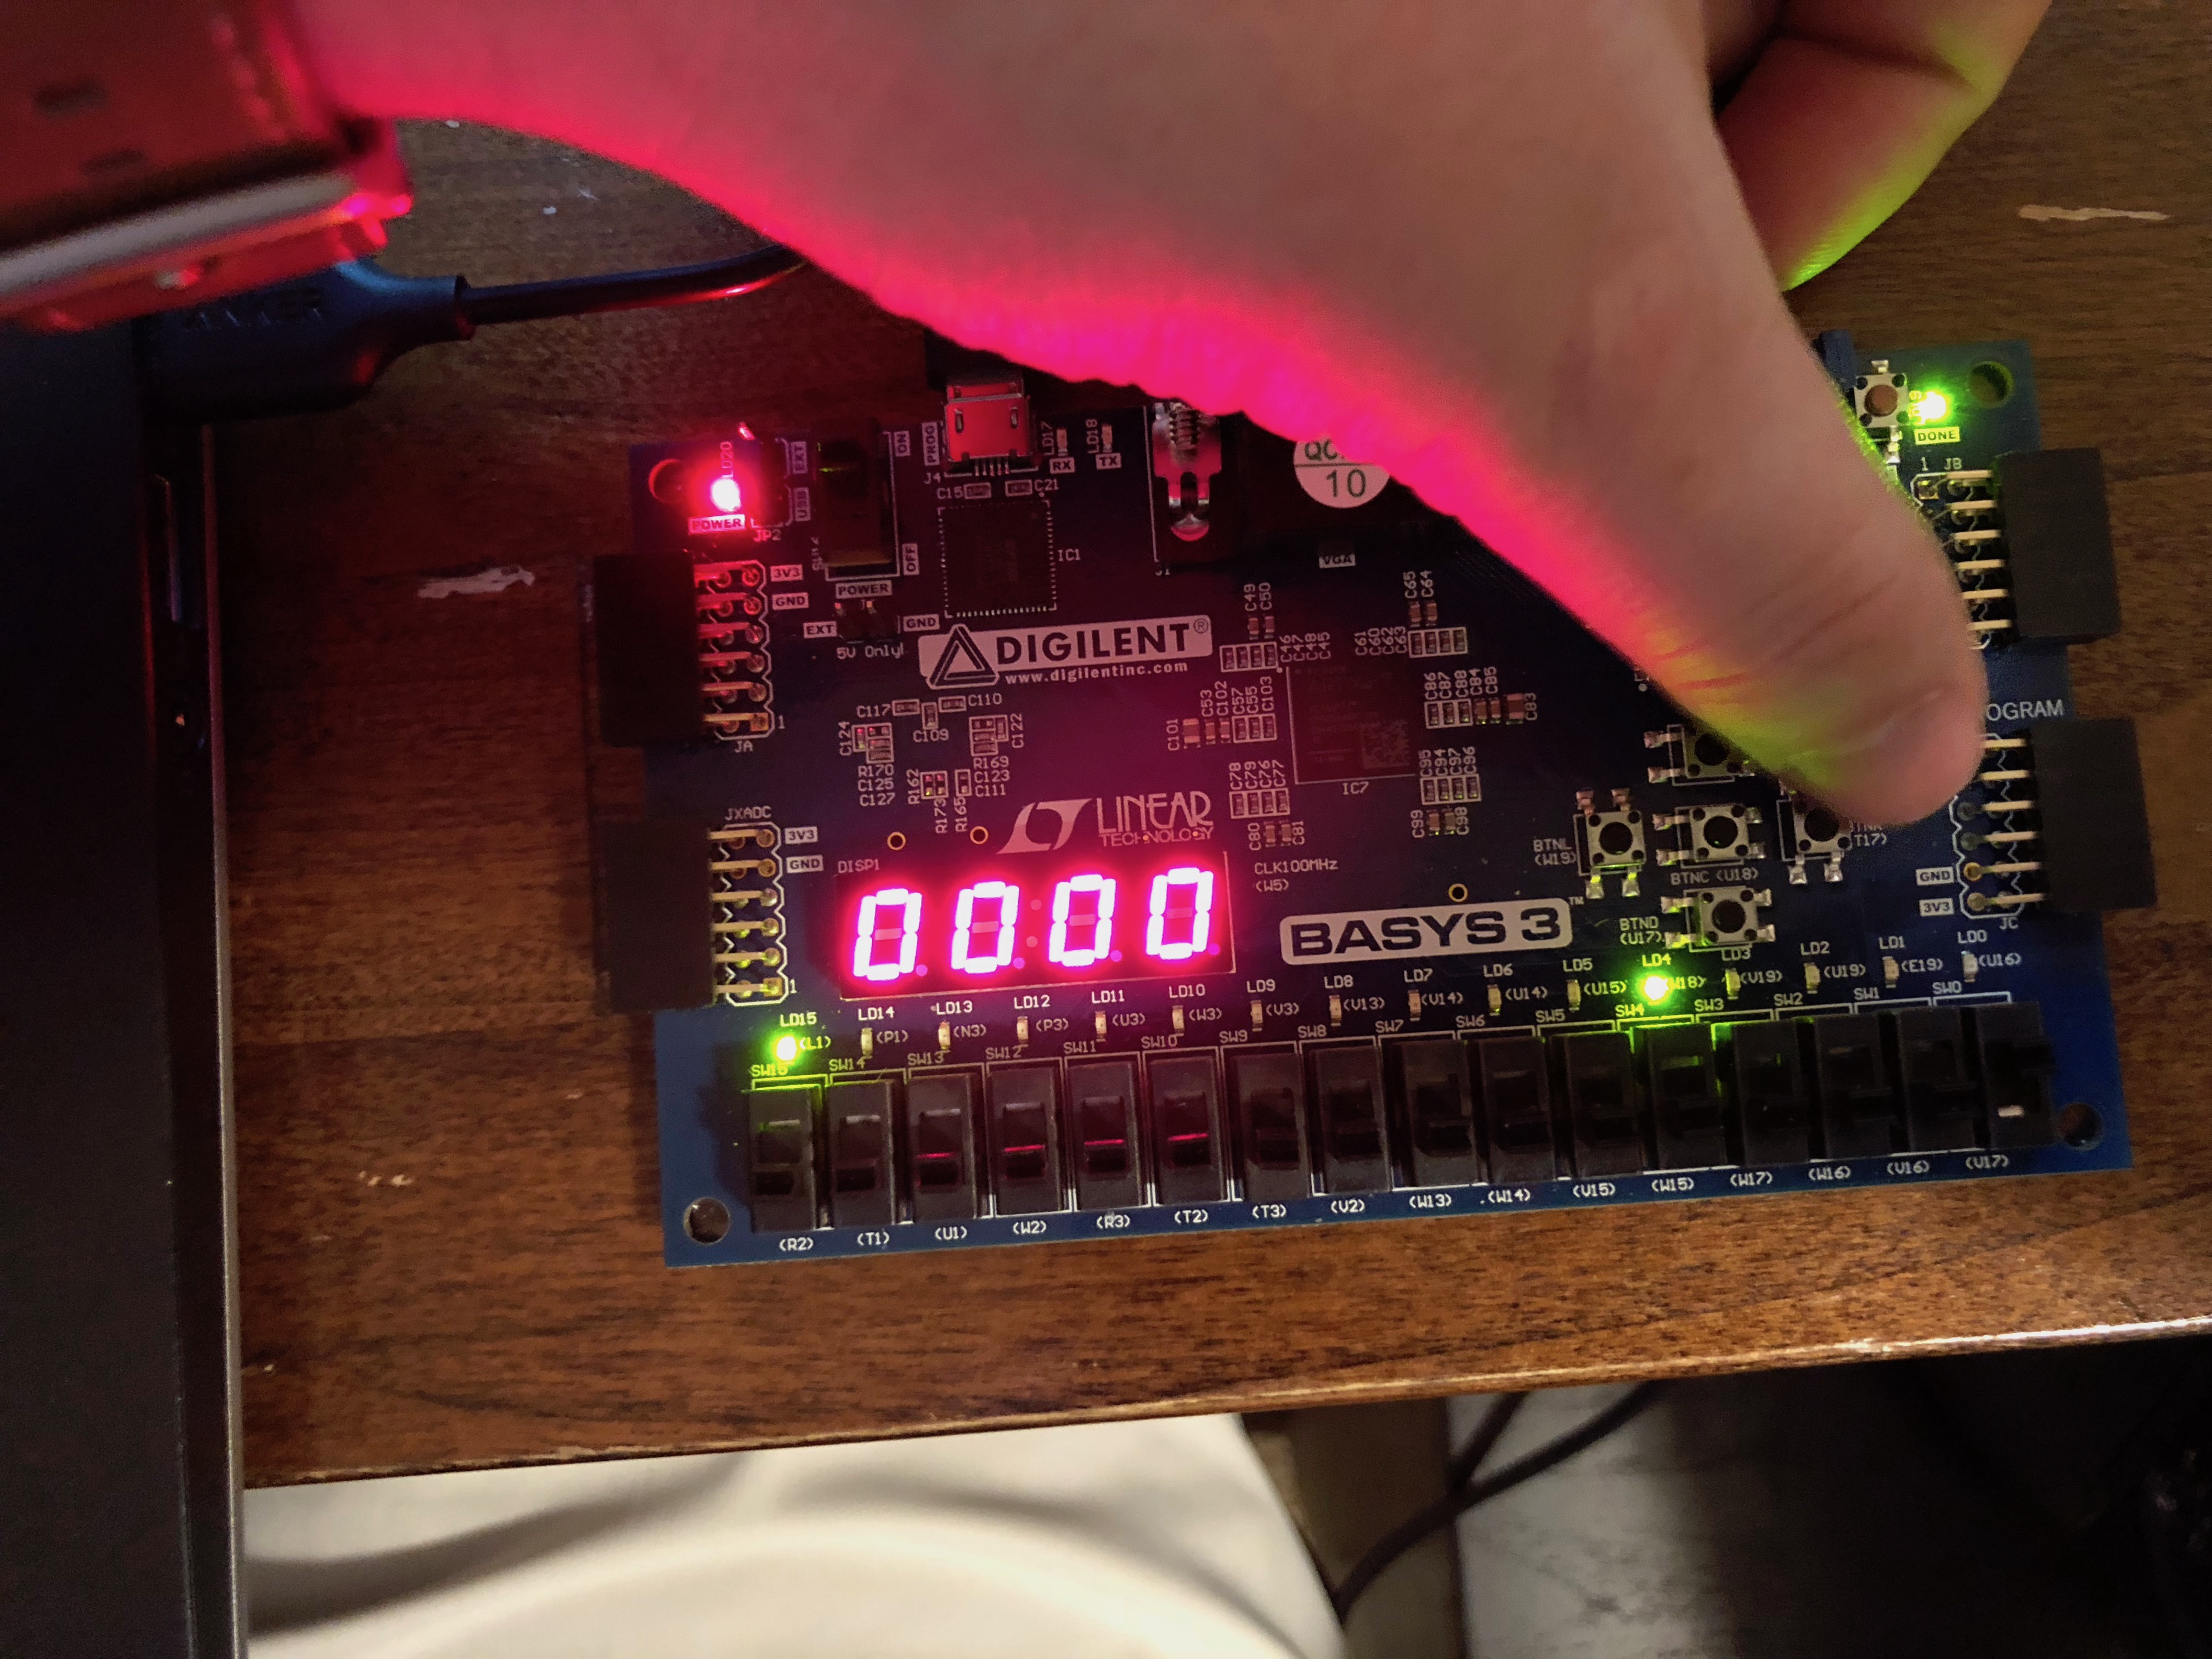
\includegraphics[width=0.5\textwidth]{./images/Part3/IMG_0588.jpg}
	\caption{\label{fig:part3img6}This image shows the state machine after receiving input '0' from State 2, which has caused it to move to State 4.}
\end{figure}
\end{center}

\begin{center}
\begin{figure}[H]
	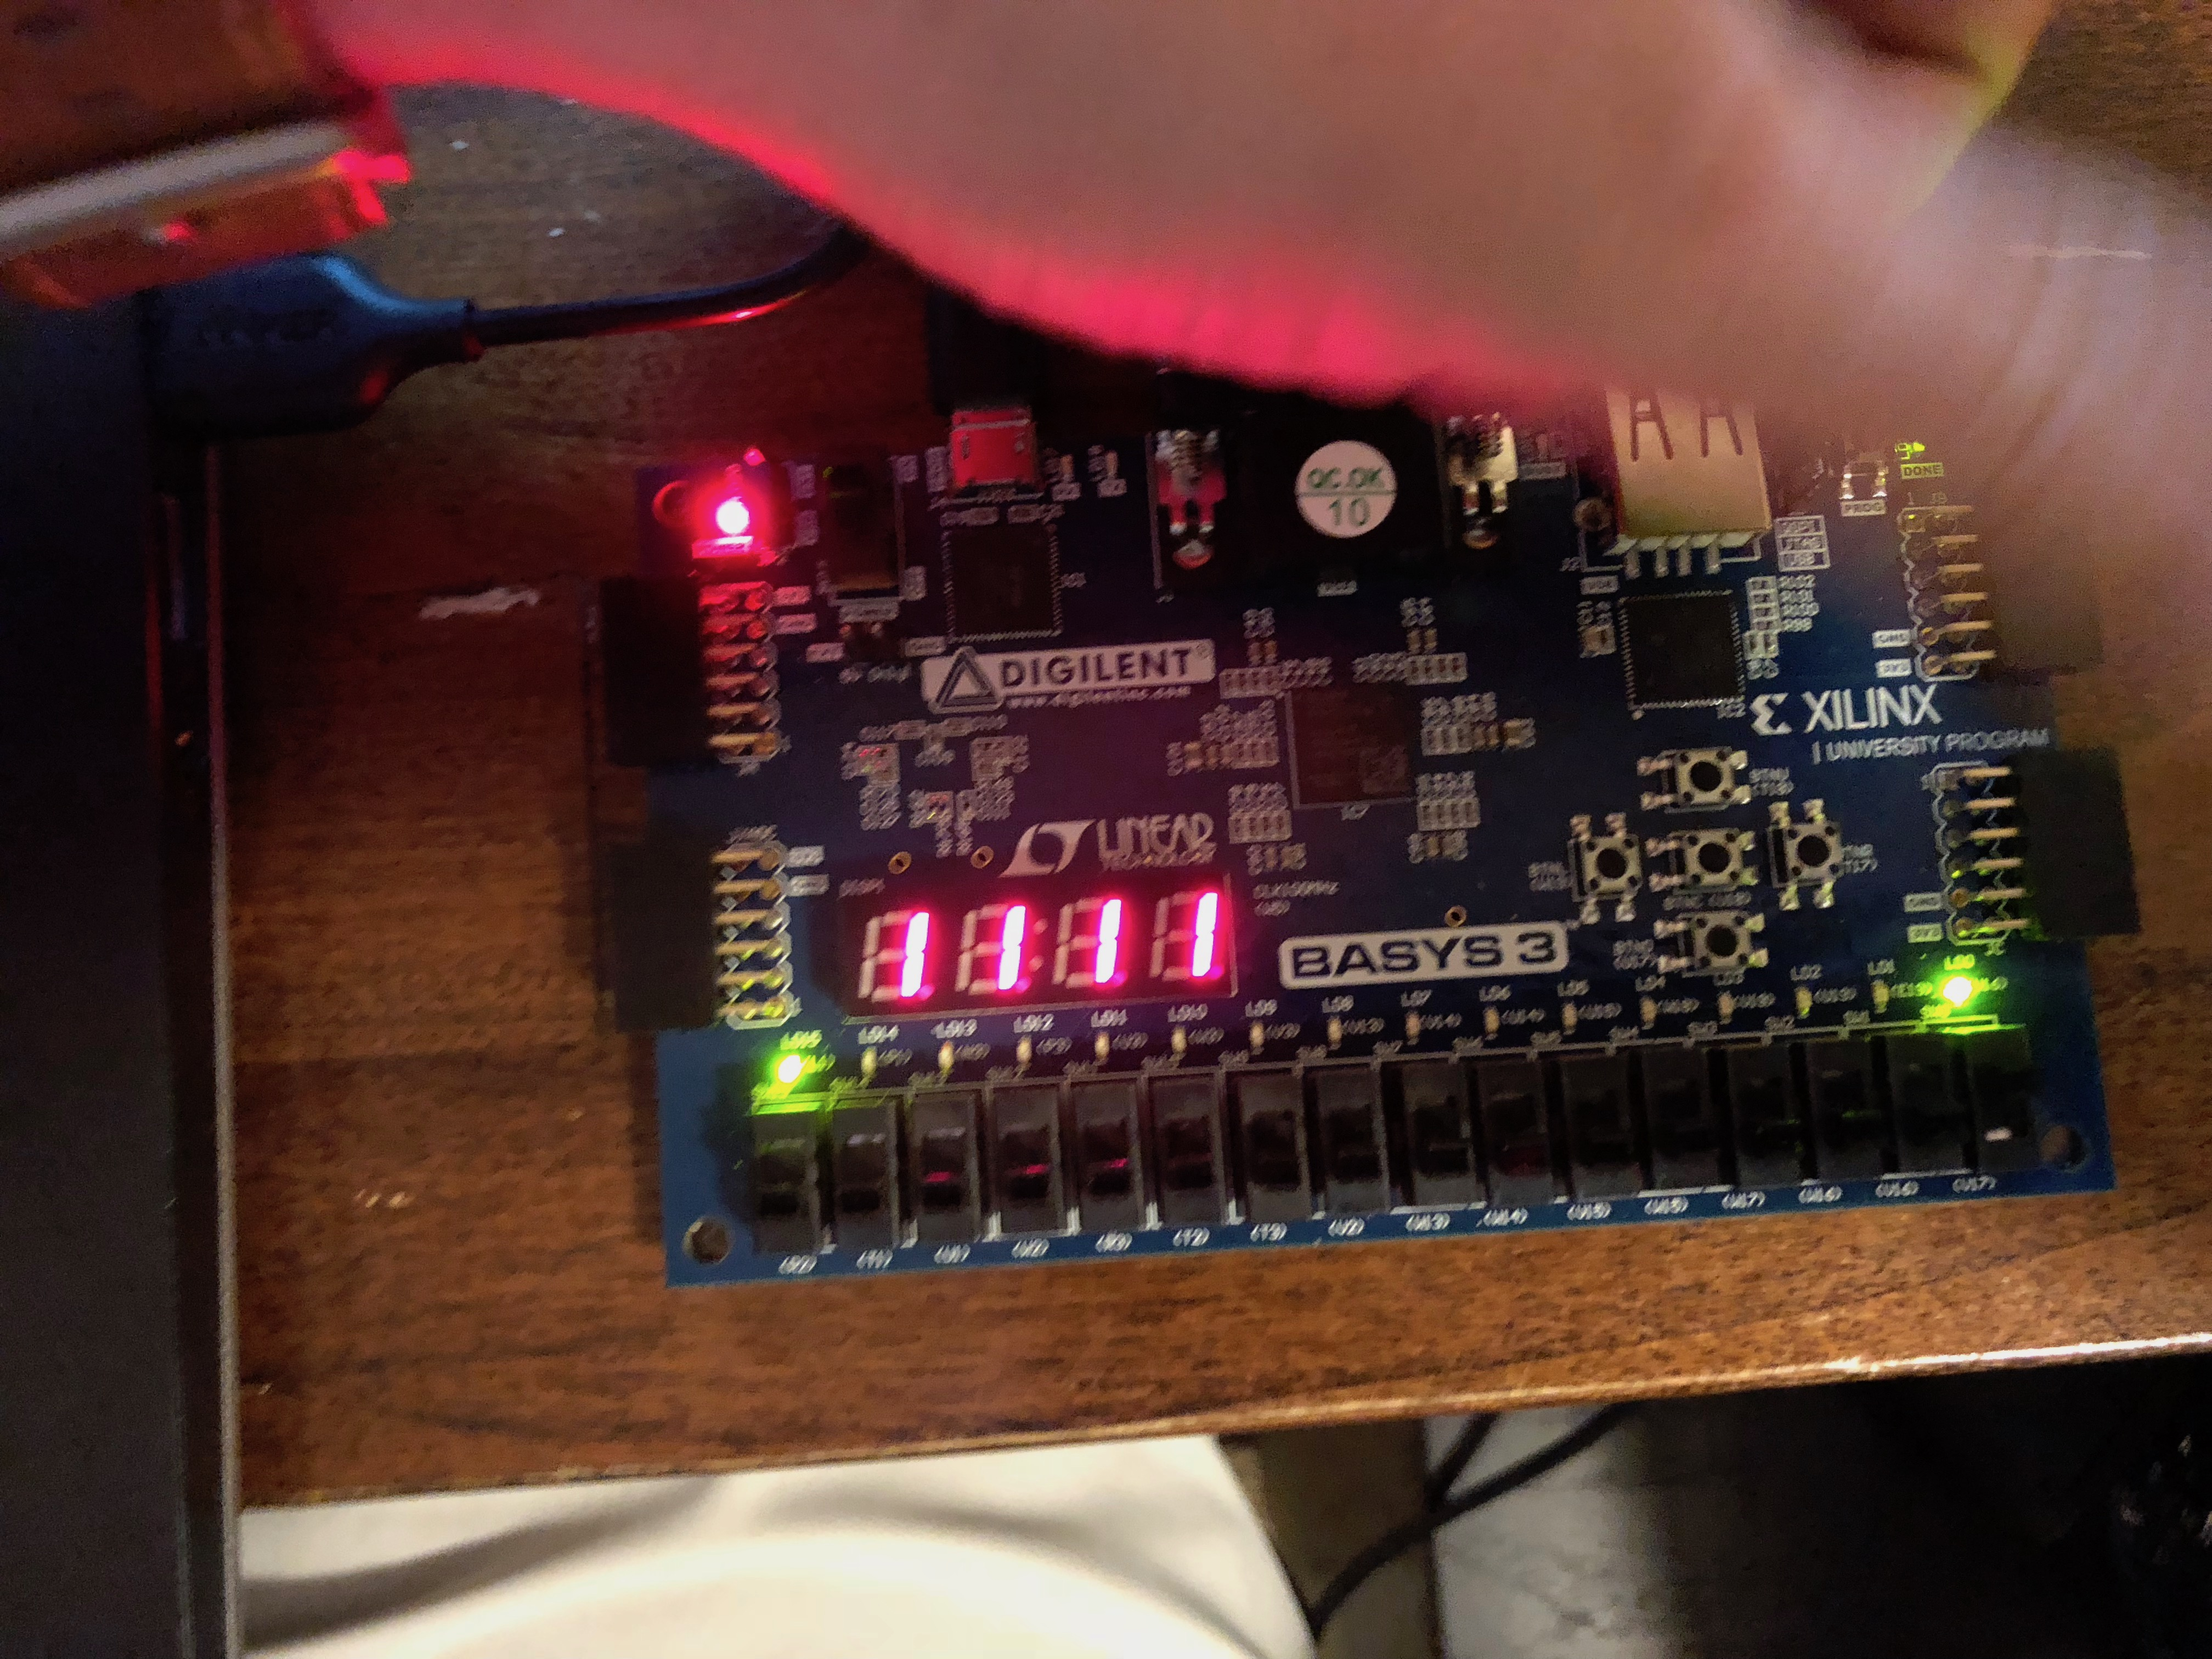
\includegraphics[width=0.5\textwidth]{./images/Part3/IMG_0589.jpg}
	\caption{\label{fig:part3img7}This image shows the state machine after receiving input '1' from State 4, so it has returned to State 0 and output 1.}
\end{figure}
\end{center}

\section{Conclusion}
In conclusion, by completing this lab we learned the implementation details of Mealy and Moore state machines in VHDL. This will be important for many tasks in digital system design. The most significant challenge for this lab was designing the Mealy State Machine for two potential sequences, but by carefully diagramming them together we were able to complete a design. State machines are essential building blocks of digital circuits, and now that we have completed them we can move on to even more advanced design.

\pagebreak

\textbf{Appendices}

\begin{appendices}

\section{Problem 1 VHDL Code}

\begin{lstlisting}[language=VHDL]
library IEEE;
use IEEE.STD_LOGIC_1164.ALL;
use IEEE.NUMERIC_STD.ALL;

--Declares clock divider entity 
entity Clockdivider is
     port(clk : in std_logic;
          start_timer : in std_logic;
	  FastClock,MediumClock,SlowClock, led0 : out std_logic);
end Clockdivider;

architecture clockdivider_arch of Clockdivider is

signal slowClock_sig : STD_LOGIC;

begin
    process 
    --When this variable reaches the most significant bit,
    --approvimately 1 second will have passes 
    variable cnt :	std_logic_vector(26 downto 0):= 
    		"000000000000000000000000000";
    begin					 
    		-- wait for a rising clock edge
        wait until ((clk'EVENT) AND (clk = '1'));
	       
	     --Reset the count variable
		if (start_timer = '1') then
	       cnt := "000000000000000000000000000";
	    else  
	    	  --Increments the count variable
           cnt := STD_LOGIC_VECTOR(unsigned(cnt) + 1);
	    end if;

   	    FastClock <= cnt(22);
   	    MediumClock <= cnt(24);	
   	    SlowClock <= cnt(26);
        slowClock_sig <= cnt(26);
	
	   --Ties LED 0 to slowClock
        if (slowClock_sig = '1') then
		  led0 <= '1';
	    else
		  led0 <= '0';
	    end if;
	end process;
end clockdivider_arch;
\end{lstlisting}

\section{Problem 1 Constraints File}
\begin{center}
\begin{figure}[H]
	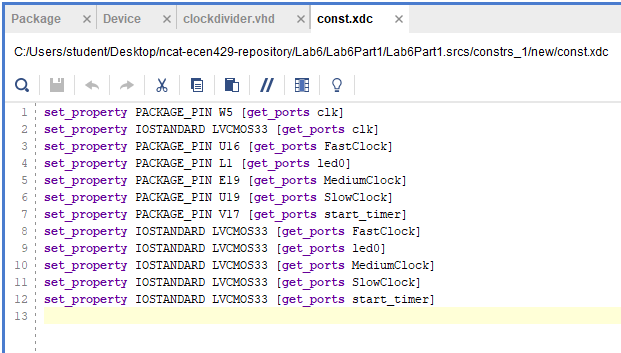
\includegraphics[scale=1]{./images/Lab6Part1Const.png}
	\caption{\label{fig:Prob1Const}Constraints file for Problem 1.}
\end{figure}
\end{center}

\section{Problem 2 VHDL Code}
\begin{lstlisting}[language=VHDL]
library IEEE;
use IEEE.STD_LOGIC_1164.ALL;
use IEEE.NUMERIC_STD.ALL;

--Declares the Moore Machine entity
entity moore_machine is
    Port ( input : in STD_LOGIC;
           clk : in STD_LOGIC;
           enable : in STD_LOGIC;
           timer_restart : in STD_LOGIC;
           reset : in STD_LOGIC;
           led0 : out STD_LOGIC;
           state : out STD_LOGIC_VECTOR(9 downto 0);
           output : out STD_LOGIC_VECTOR(6 downto 0));
end moore_machine;

architecture moore_arch of moore_machine is
--Declares a component to slow down the clock
component Clockdivider is
    Port ( clk : in STD_LOGIC;
           start_timer : in STD_LOGIC;
           FastClock,MediumClock,SlowClock,led0 : out STD_LOGIC);
end component Clockdivider;

signal slowClock : STD_LOGIC;
signal mediumClock : STD_LOGIC;
signal fastClock : STD_LOGIC;
signal current_state : STD_LOGIC_VECTOR(3 downto 0) := "0000";

begin  
	--Instantiates the clock divider component
    clock : Clockdivider port map(clk, timer_restart, fastClock, mediumClock, 
    		slowClock, led0);
    process(slowClock, enable)
    begin
    	   --Reset will set back to State '0'
        if(reset = '1') then current_state <= "0000";
        end if;
        --Looks for a rising slow clock edge
        if(slowClock'event and (slowClock = '1')) then
		  --Progresses the state machine with an input of '1'           
            if(enable = '1') then
                if(current_state = "1001") then
                    current_state <= "0000";
                else
                    current_state <= std_logic_vector
                    		( unsigned(current_state) + 1 );
                end if;
            else current_state <= "0000";
            end if;
        end if;
    end process;
    process(current_state)
    	
    begin
    	  --Will output based on state diagram
        if((current_state = "0100") or (current_state = "1000")) then
            output <= "1001111";
        else
            output <= "1000000";
        end if;
        --Displays the state on the LEDs 
        case current_state is
            when "0000" => state <= "0000000001";
            when "0001" => state <= "0000000010";
            when "0010" => state <= "0000000100";
            when "0011" => state <= "0000001000";
            when "0100" => state <= "0000010000";
            when "0101" => state <= "0000100000";
            when "0110" => state <= "0001000000";
            when "0111" => state <= "0010000000";
            when "1000" => state <= "0100000000";
            when "1001" => state <= "1000000000";
            when others => state <= "0000000000";
        end case;
    end process;
end moore_arch;

\end{lstlisting}

\section{Problem 2 Constraints File}
\begin{center}
\begin{figure}[H]
	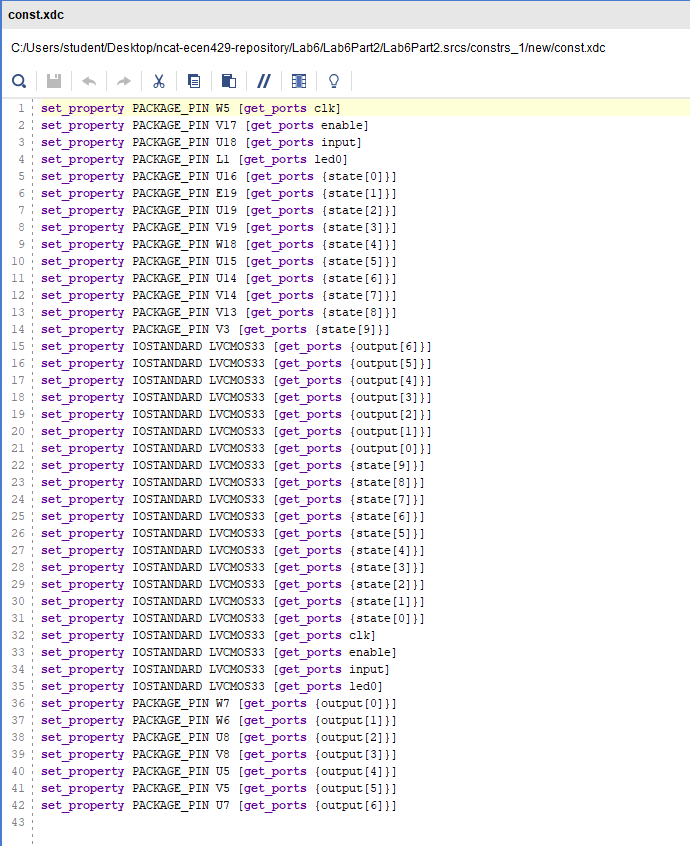
\includegraphics[scale=1]{./images/Lab6Part2Const.png}
	\caption{\label{fig:Prob1Const}Constraints file for Problem 2.}
\end{figure}
\end{center}

\section{Problem 3 VHDL Code}
\begin{lstlisting}[language=VHDL]
library IEEE;
use IEEE.STD_LOGIC_1164.ALL;

--Declares the Mealy Machine entity
entity mealy is
    Port ( clk : in STD_LOGIC;
           enable : in STD_LOGIC;
           clock_reset : in STD_LOGIC;
           reset : in STD_LOGIC;
           input : in STD_LOGIC;
           led0 : out STD_LOGIC;
           output : out STD_LOGIC_VECTOR(6 downto 0);
           state : out STD_LOGIC_VECTOR(4 downto 0));
end mealy;

architecture Behavioral of mealy is
--Declares a clock divider component
component Clockdivider is
    Port ( clk : in STD_LOGIC;
           start_timer : in STD_LOGIC;
           FastClock,MediumClock,SlowClock,led0 : out STD_LOGIC);
end component Clockdivider;

signal slowClock : STD_LOGIC;
signal mediumClock : STD_LOGIC;
signal fastClock : STD_LOGIC;
signal current_state : STD_LOGIC_VECTOR(2 downto 0) := "000";
signal output_signal : STD_LOGIC := '0'; 

begin
	--Instantiates the clock divider
    clock : Clockdivider port map(clk, clock_reset, fastClock, mediumClock, 
    		slowClock, led0);
    process(slowClock, enable)
    begin
    		--Sets back to State 0 if reset
        if(reset = '1') then current_state <= "000";
        end if;
        --Waits for a slow clock rising edge
        if(slowClock'event and (slowClock = '1')) then
            if(enable = '1') then
            	  --Evaluates current state and current input,
            	  --Updates next state and output signal accordingly
                case current_state is
                    when "000" =>
                        if(input = '1') then 
                            current_state <= "010";
                            output_signal <= '0';
                        else 
                            current_state <= "001";
                            output_signal <= '0';
                        end if;
                    when "001" =>
                        if(input = '1') then 
                            current_state <= "011";
                            output_signal <= '0';
                        else
                            current_state <= "001";
                            output_signal <= '0';
                        end if;
                    when "010" =>
                        if(input = '1') then 
                            current_state <= "010";
                            output_signal <= '0';
                        else
                            current_state <= "100";
                            output_signal <= '0';
                        end if;
                    when "011" =>
                        if(input = '1') then 
                            current_state <= "010";
                            output_signal <= '0';
                        else
                            current_state <= "000";
                            output_signal <= '1';
                        end if;
                    when others =>
                        if(input = '1') then 
                            current_state <= "000";
                            output_signal <= '1';
                        else
                            current_state <= "001";
                            output_signal <= '0';
                        end if;
                end case;
            else
                current_state <= "000";
                output_signal <= '0';
            end if;
        end if;
    end process;
    process(output_signal)
    begin
    	  --Set s the output based on an output signal
        if(output_signal = '1') then
            output <= "1001111";
        else
            output <= "0000001";
        end if;
    end process;
    process(current_state)
    begin
    	   --Ties state to LED indicators
        case current_state is
            when "000" => state <= "00001";
            when "001" => state <= "00010";
            when "010" => state <= "00100";
            when "011" => state <= "01000";
            when "100" => state <= "10000";
            when others => state <= "00000";
        end case;
    end process;
end Behavioral;
\end{lstlisting}

\section{Problem 3 Constraints File}
\begin{center}
\begin{figure}[H]
	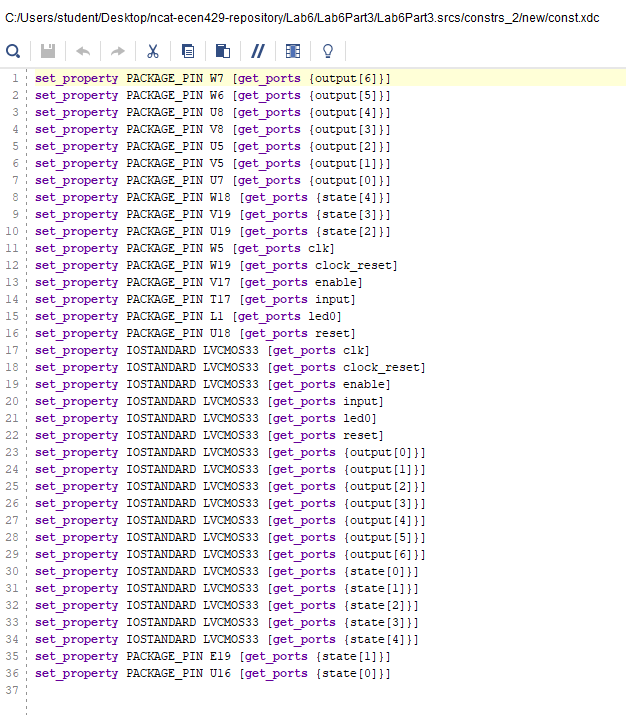
\includegraphics[scale=1]{./images/Lab6Part3Const.png}
	\caption{\label{fig:Prob1Const}Constraints file for Problem 3.}
\end{figure}
\end{center}

\end{appendices}
\end{document}
